%%%%%%%%%%%%%%%%%%%%%%%%%%%%%%%%%%%%%%%%%%%%%%%%%%%%%%%%%
%%             东南大学数电实验报告 LaTeX 模板
%%               Experiment 3 Report.tex
%% https://github.com/Teddy-van-Jerry/SEU_Digital_Report
%% ======================================================
%% 版本信息:
%% v1.0 (Nov. 07, 2021)
%% ------------------------------------------------------
%% 模板制作:
%% Teddy van Jerry, (me@teddy-van-jerry.org)
%% * GitHub: https://github.com/Teddy-van-Jerry
%% * Website: https://teddy-van-jerry.org
%% * Blog: https://blog.teddy-van-jerry.org
%% ------------------------------------------------------
%% 使用说明:
%% 1. 编译使用 XeLaTeX 和 Biber
%% 2. 报告基本信息通过修改导言区以 exp 开头的命令
%% 3. 参考文献位于 ref/ref.bib
%% 4. 报告模板依据 MIT License 开源共享
%% ------------------------------------------------------
%% Copyright 2021 (c) Teddy van Jerry
%%
%% Permission is hereby granted, free of charge, to any
%% person obtaining a copy of this software and
%% associated documentation files (the "Software"), to
%% deal in the Software without restriction, including
%% without limitation the rights to use, copy, modify,
%% merge, publish, distribute, sublicense, and/or sell
%% copies of the Software, and to permit persons to whom
%% the Software is furnished to do so, subject to the
%% following conditions:
%%
%% The above copyright notice and this permission notice
%% shall be included in all copies or substantial
%% portions of the Software.
%% 
%% THE SOFTWARE IS PROVIDED "AS IS", WITHOUT WARRANTY OF
%% ANY KIND, EXPRESS OR IMPLIED, INCLUDING BUT NOT
%% LIMITED TO THE WARRANTIES OF MERCHANTABILITY, FITNESS
%% FOR A PARTICULAR PURPOSE AND NONINFRINGEMENT. IN NO
%% EVENT SHALL THE AUTHORS OR COPYRIGHT HOLDERS BE LIABLE
%% FOR ANY CLAIM, DAMAGES OR OTHER LIABILITY, WHETHER IN
%% AN ACTION OF CONTRACT, TORT OR OTHERWISE, ARISING
%% FROM, OUT OF OR IN CONNECTION WITH THE SOFTWARE OR THE
%% USE OR OTHER DEALINGS IN THE SOFTWARE.
%%%%%%%%%%%%%%%%%%%%%%%%%%%%%%%%%%%%%%%%%%%%%%%%%%%%%%%%%%

%% 使用实验报告模板类(字体大小 11pt 约为五号字)
\documentclass[11pt]{SEU-Digital-Report}

%%%%%%%%%%%%%%%%%%%% 报告基本信息 %%%%%%%%%%%%%%%%%%%%
\expno{三} % 实验序号
\expname{时序逻辑与设计} % 实验名称
\expauthor{赵舞穹} % 姓名
\expID{61520522} % 学号
\expmates{郑瑞琪} % 同组
\expmatesID{61520523} % 学号(同组)
\expmajor{工科试验班} % 专业
\explab{计算机硬件技术} % 实验室
\expdate{2021年11月12日} % 实验日期
\expreportdate{\today} % 实验日期
\expgrade{} % 成绩评定
\exptutor{冯熳} % 评阅教师
%%%%%%%%%%%%%%%%%%%%%%%%%%%%%%%%%%%%%%%%%%%%%%%%%%%%

\usepackage{pgfplots}
\pgfplotsset{compat=1.11}

%% 报告正文
\begin{document}
  % 打印封面页
  \exptitlepage

  \tableofcontents
  \newpage

  \section{实验目的与内容}

  % http://www.diyleyuan.com/JC/162.html
        
    \begin{enumerate}
        \item 进一步熟悉数字逻辑与硬件接口基本实验仪器的使用及TPC 实验装置中基本数字
        逻辑单元的基本原理和组成结构, 学会利用开关输入/LED 发光管/8 段数码管输出电路及示
        波器、电平逻辑笔等验证测试组合逻辑基本特性;
        \item 分析掌握TPC 实验装置板上74LS74(双D 触发器,带置位/清零端)、74LS273(8
        位寄存器,边沿触发带清零端)、扩展CD4518(双BCD 加计数器)等时序逻辑电路模块的
        工作原理,设计实验方案,配接开关电平转换、LED 发光管驱动、与或非门等组合逻辑电
        路,搭建应用实验系统,完成接线、演示功能及特性验证;
        \item 正确认识HDL 阻塞与非阻塞赋值语句、\texttt{always@}语句(块)的正确使用,学习掌握
        FPGA 数字系统基本触发器、锁存器、计数器、移位器的数据流和行为描述的HDL 模型开
        发方法,收集构建基本模块资源;
        \item 完成典型时序逻辑实验电路及测试(\texttt{initial})模块的HDL 模型搭建、模块编程、配
        置、调试、分析环节,完成仿真运行分析和输入输出演示实验,掌握基于工具软件的时序
        逻辑设计概念和设计流程,为后续复杂可编程数字模块逻辑设计打下基础. 
    \end{enumerate}

    \section{基本实验原理}

      \begin{device}{}{devices}
        \begin{itemize}
          \item 清华科教仪器厂TPC-ZK-II\_PCI 微机接口实
          验装置
          \item EEEC-020A 计算机组成实验箱一台(自带电压表)
          \item RIGAL DG1022U 25MHz 双路波形发生器
          \item RIGOL DS1072E-EDU 70MHz 双踪数字记忆示波器
          \item Xilinx Vivado \textit{HLx} 2017.4
          \item Ubuntu 20 / Windows 11 (x86\_64){\kaishu\color{gray}(主要实验于 Ubuntu 平台完成)}
          \item 没有具体的开发板,仅限于线上仿真和使用 Verilog 进行电路设计
        \end{itemize}
      \end{device}

      \newpage
      \subsection{7474逻辑电路}

        7474(D Flip Flop)逻辑电路如图~\ref{fig:74LS74_module}~所示,其中 CD 为 clear,SD 为 set,均为低电平有效.
        其真值表见图~\ref{tab:74LS74_tt}.

        \begin{figure}[htbp]
          \centering
          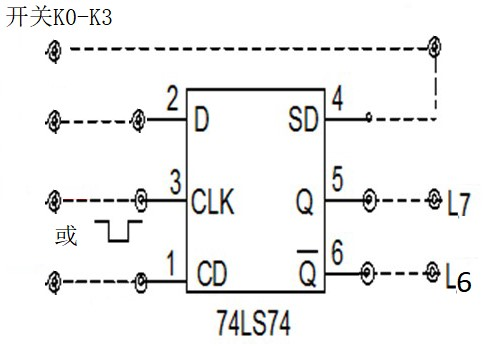
\includegraphics[width=.4\linewidth]{fig/74LS74_module.jpg}
          \caption{74LS74 引脚示意图\cite{guide}}
          \label{fig:74LS74_module}
        \end{figure}
        \begin{table}[htbp]
          \centering
          \caption{74LS74 真值表\cite{ppt3}}
          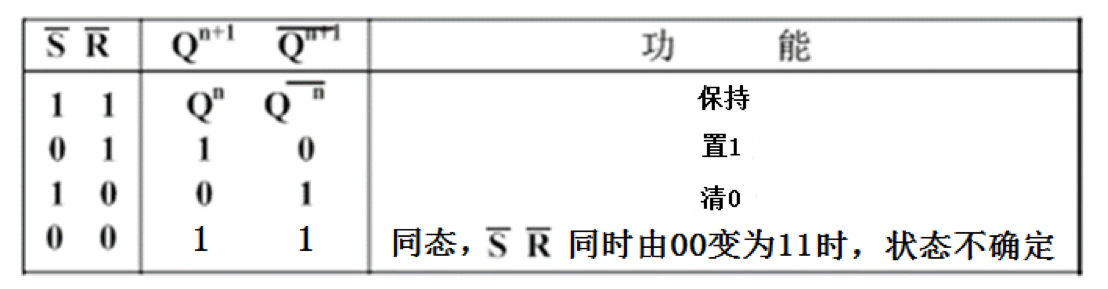
\includegraphics[width=.5\linewidth]{fig/74LS74_tt.png}
          \label{tab:74LS74_tt}
        \end{table}

      \subsection{8 位数据/地址锁存器(8D 触发器)}

      74LS273 是8 位数据/地址锁存器,它是一种带清除功能的8D 触发器. 接线如图~\ref{fig:74LS273_module}~,
利用实验箱简单输入接口实验区的三态总线缓冲器74LS273.

        \begin{figure}[htbp]
          \centering
          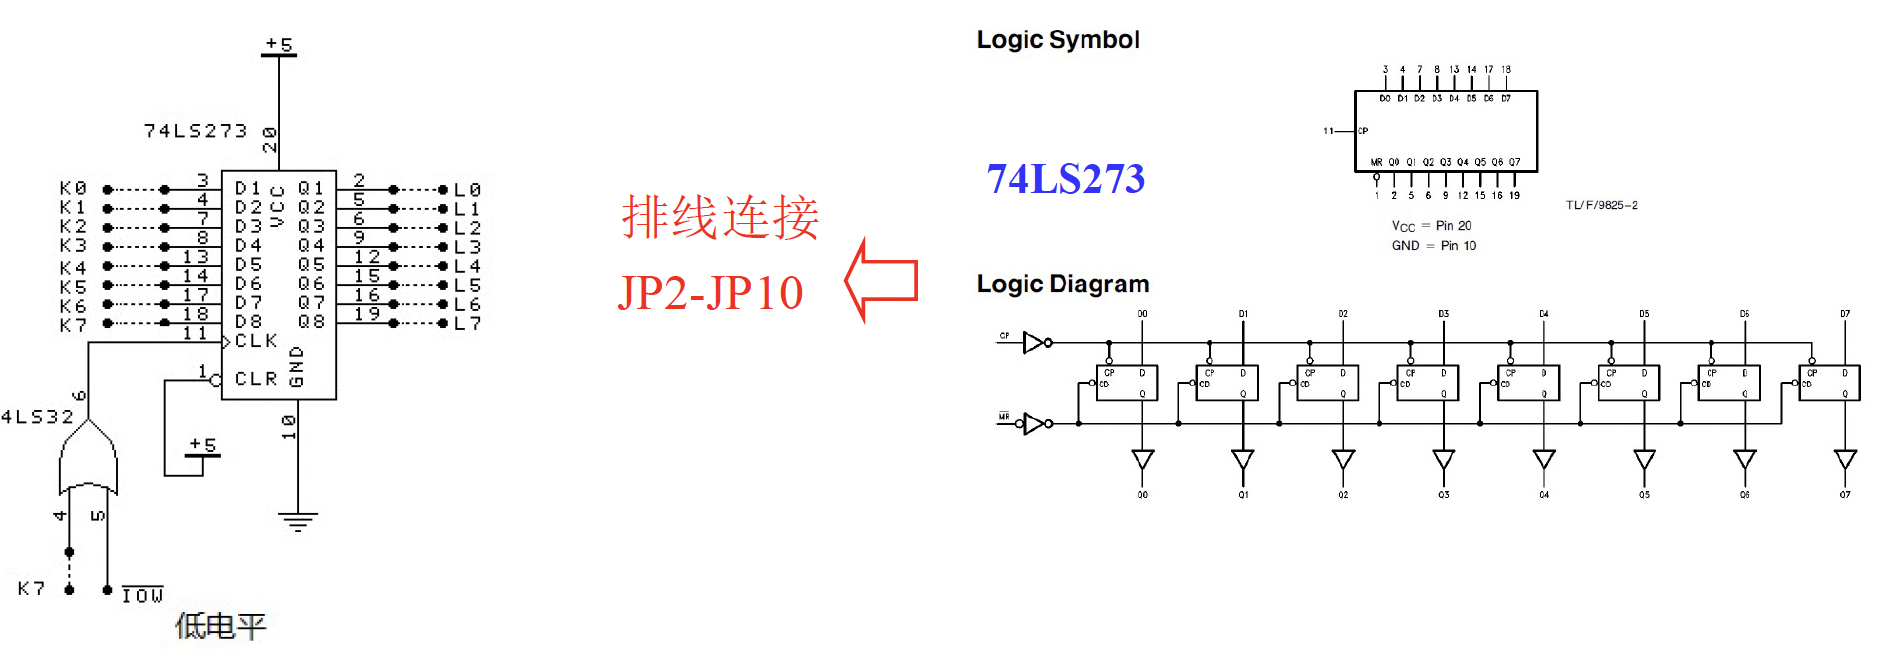
\includegraphics[width=.8\linewidth]{fig/74LS273_module.png}
          \caption{74LS273接线图}
          \label{fig:74LS273_module}
        \end{figure}

        \newpage
    \subsection{双8 位数据/地址锁存器(8D 触发器)}

        使用实例见图~\ref{fig:8x8_}.

    \begin{figure}[htbp]
      \centering
      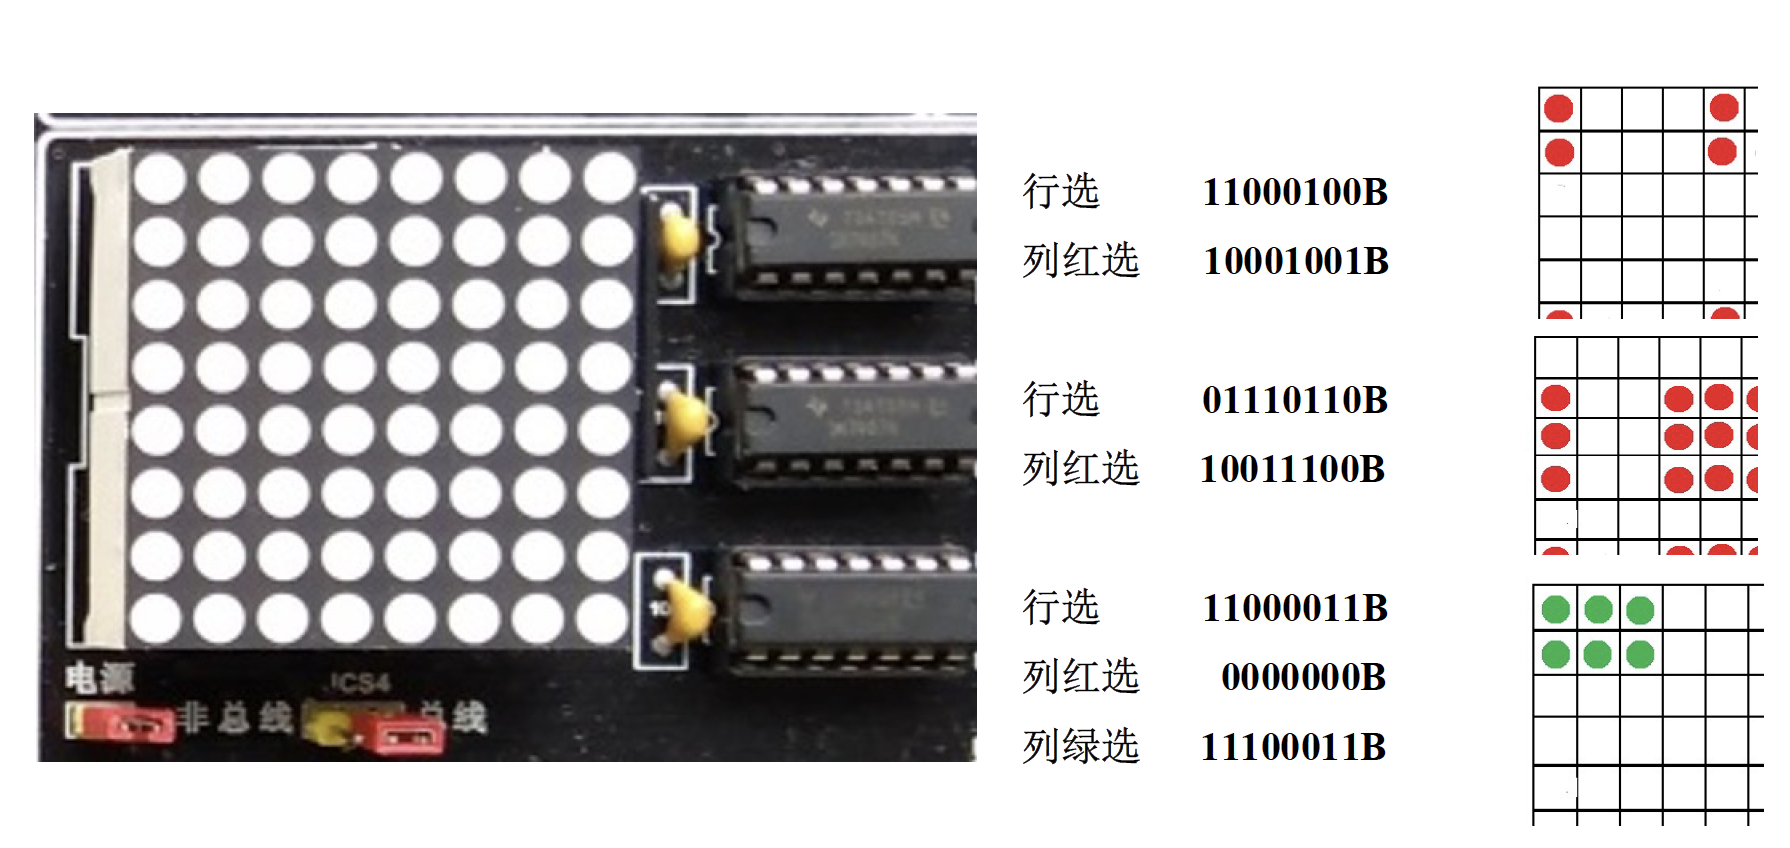
\includegraphics[width=.8\linewidth]{fig/8x8_.png}
      \caption{双74LS273 输出($8\times 8$点阵显示)}
      \label{fig:8x8_}
    \end{figure}

    原理如图~\ref{fig:8x8__}~所示. 双色点阵在列红选为000000000B 时列绿选才有效. 动态显示可
    以实现各种图形文字效果,如“年”字显示(如图).
    \begin{figure}[htbp]
      \centering
      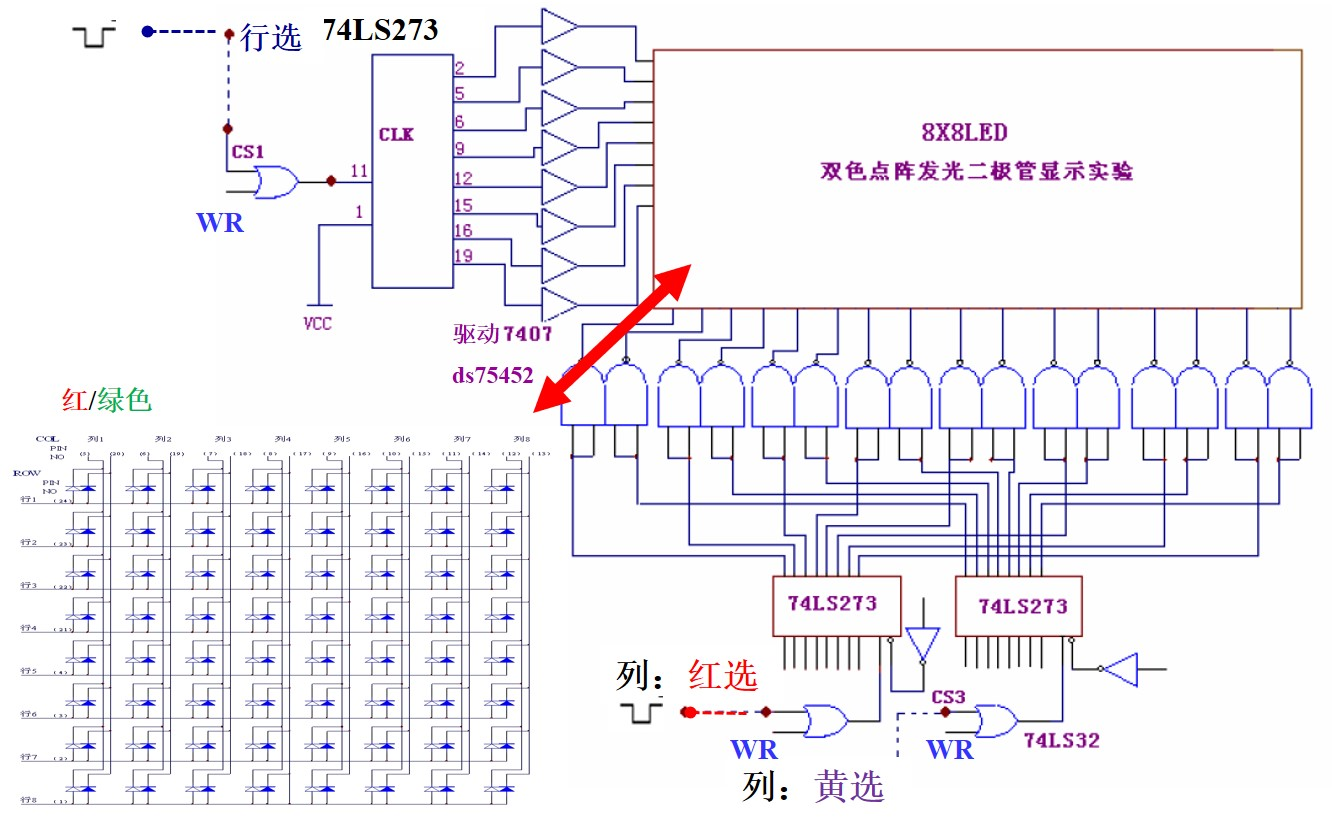
\includegraphics[width=.9\linewidth]{fig/8x8__.jpg}
      \caption{双74LS273 输出($8\times 8$点阵显示)原理}
      \label{fig:8x8__}
    \end{figure}

    \newpage
    \subsection{扩展CD4518 计数器(双BCD 加计数器)}

    CD4518BC 是一双BCD 加计数器, 引脚功能如图~\ref{fig:CD4518_module},真值表如图~\ref{subfig:CD_4518tt}. 

    \begin{figure}[htbp]
      \centering
      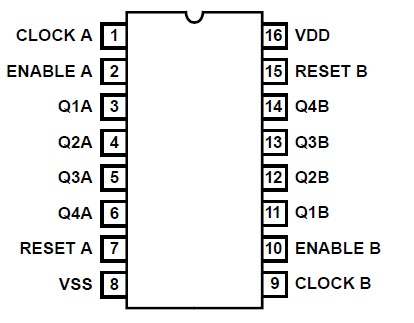
\includegraphics[width=.3\linewidth]{fig/CD4518_module1.jpg}
      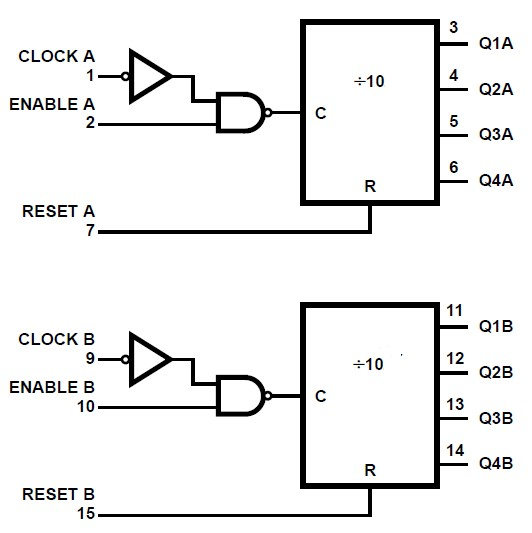
\includegraphics[width=.3\linewidth]{fig/CD4518_module2.jpg}
      \caption{CD4518 双BCD 加计数器}
      \label{fig:CD4518_module}
    \end{figure}

    \begin{figure}[htbp]
      \centering
      \subfloat[真值表]{
        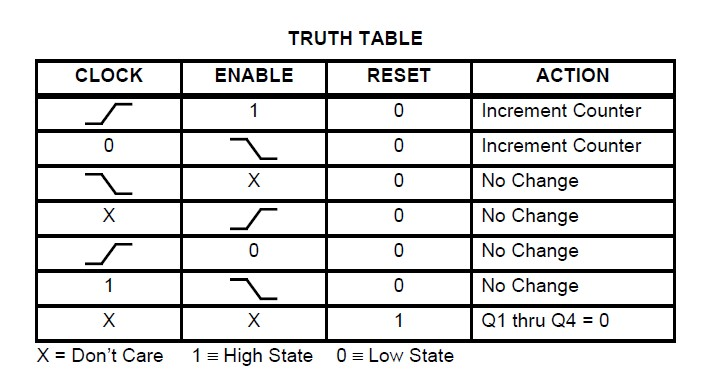
\includegraphics[width=.45\linewidth]{fig/Cd4518tt.jpg}
        \label{subfig:CD_4518tt}
      }
      \subfloat[特性波形]{
        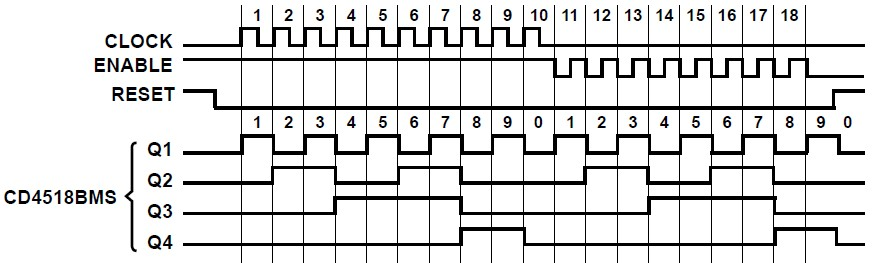
\includegraphics[width=.54\linewidth]{fig/CD4518_wave.jpg}
        \label{subfig:CD4518_wave}
      }
      \caption{CD4518 双BCD 加计数器真值表/特性波形}
    \end{figure}

    \begin{figure}[htbp]
      \centering
      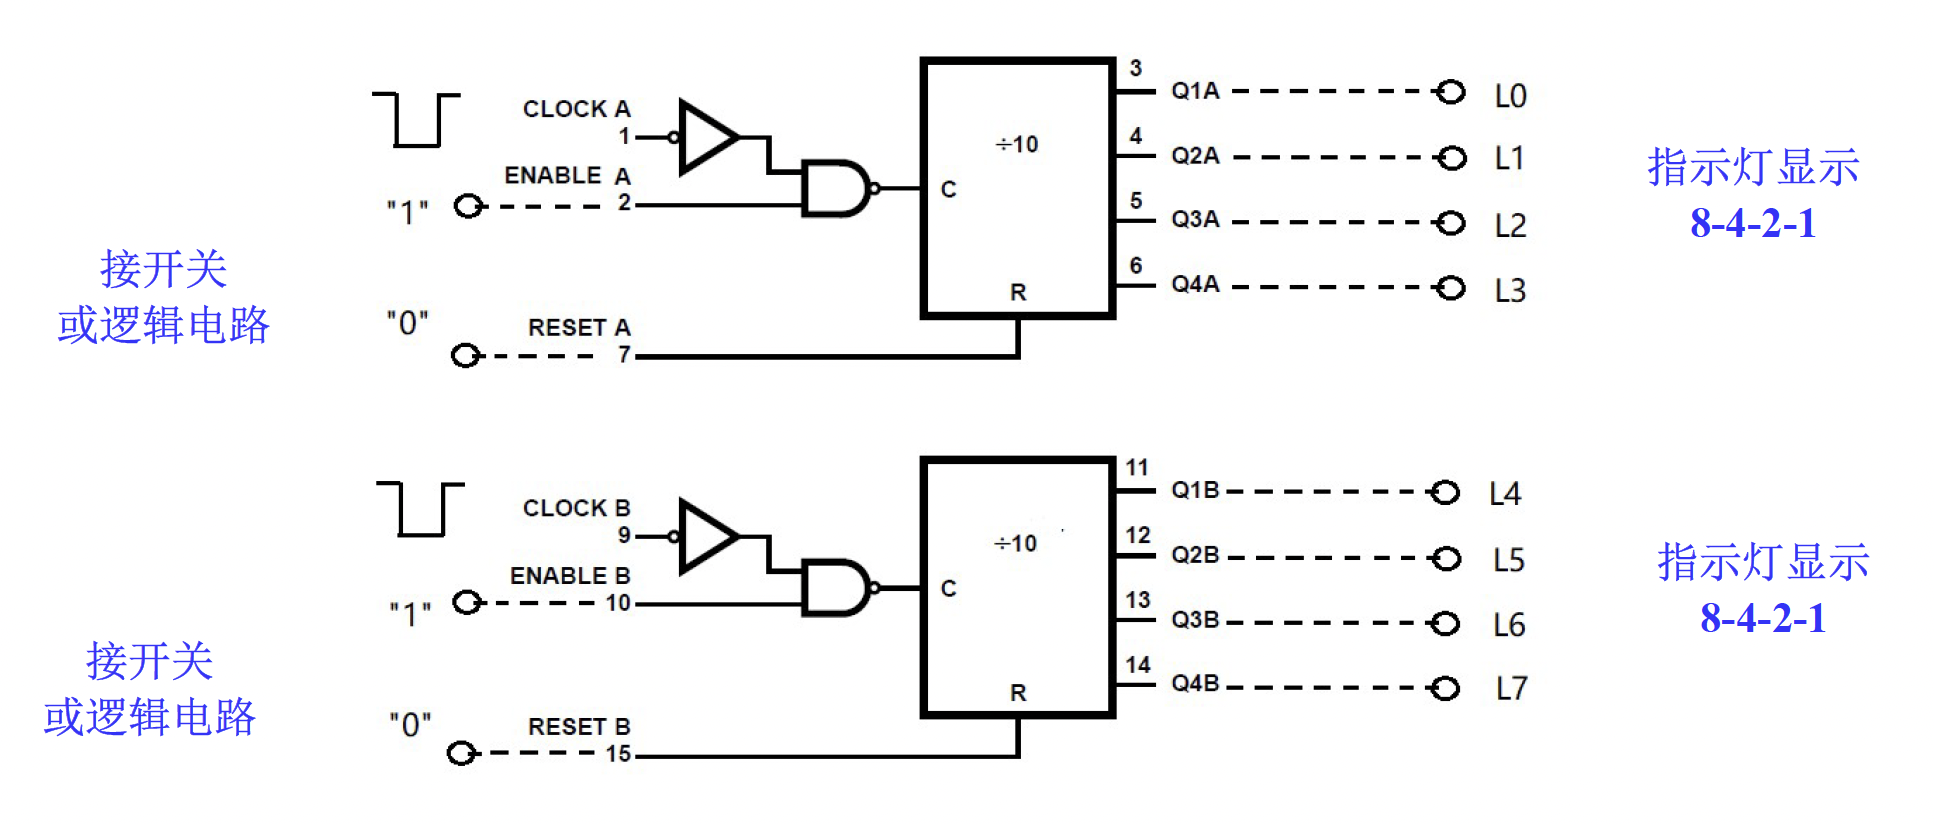
\includegraphics[width=.6\linewidth]{fig/CD4518_.png}
      \caption{CD4518 双BCD 加计数器接线图}
      \label{fig:CD4518_}
    \end{figure}

    \newpage
    \section{实验内容}

      \subsection{简单时序逻辑}

      利用实验箱上7474 逻辑电路,输入接开关,输出接指示灯. 连线,记录说明Q 输出波
形特性;

    真实连线如图~\ref{subfig:7474_real}~所示,所得输出波形为图~\ref{subfig:7474_result}.

    \begin{figure}[htbp]
      \centering
      \subfloat[真实连线图]{
        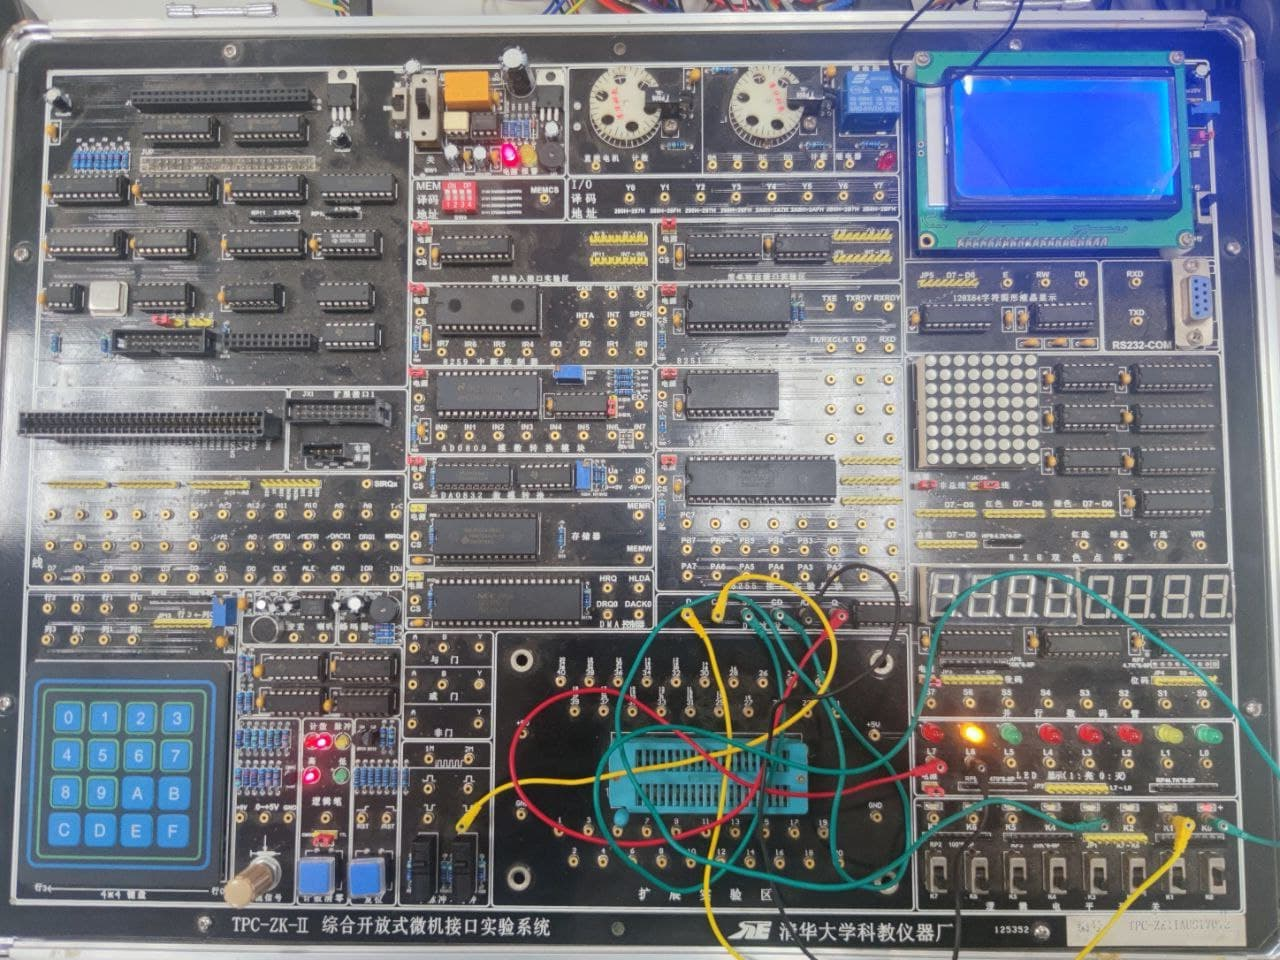
\includegraphics[width=.45\linewidth]{fig/7474_real.jpg}
        \label{subfig:7474_real}
      }
      \subfloat[Q输出波形特性]{
        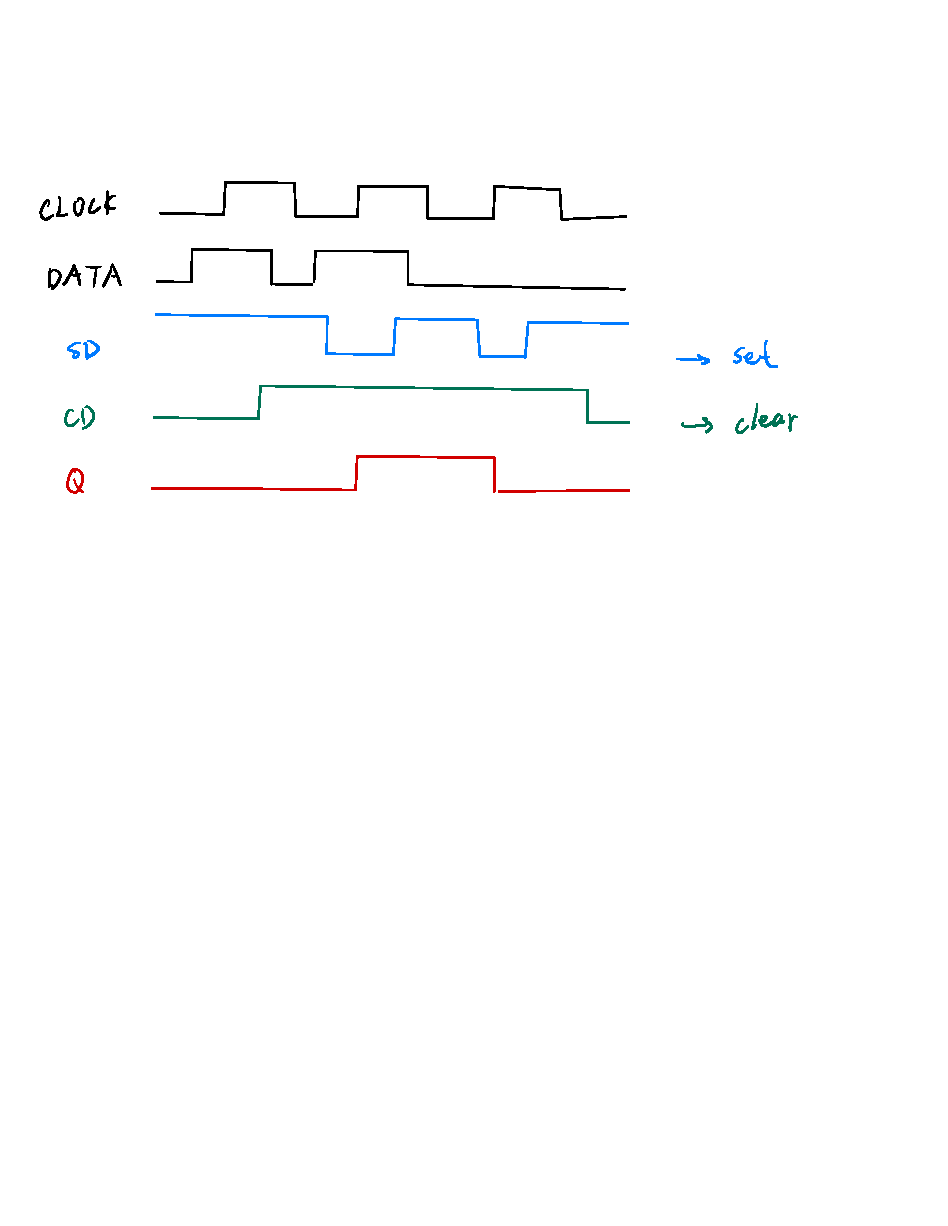
\includegraphics[width=.5\linewidth]{fig/7474_result.pdf}
        \label{subfig:7474_result}
      }
      \caption{7474简单时序逻辑}

      \begin{analyze}{简单时序逻辑}{}
        结果与预期一致,与真值表表~\ref{tab:74LS74_tt}~相符,验证了 D Flip Flop 的功能.
      \end{analyze}

    \end{figure}

      \subsection{8 位数据/地址锁存器(8D 触发器)器特性实验}

      \begin{note}{接线}{}
        断开PC 机总线D 型插座.
        排线1 一端接逻辑开关输入JP1 (K0-K7),一端接总线缓冲器输入端JP9(IN7---IN0);

      排线2 一端接总线缓冲器输出/JP10 (O7---O0),一端接LED 指示灯显示/JP2(L7---L0).
      \end{note}

      按动开关K7 控制使能端,记录示波器观察缓冲器输出(L7-L0)及指示灯状态等结果;

      \begin{figure}[htbp]
        \centering
        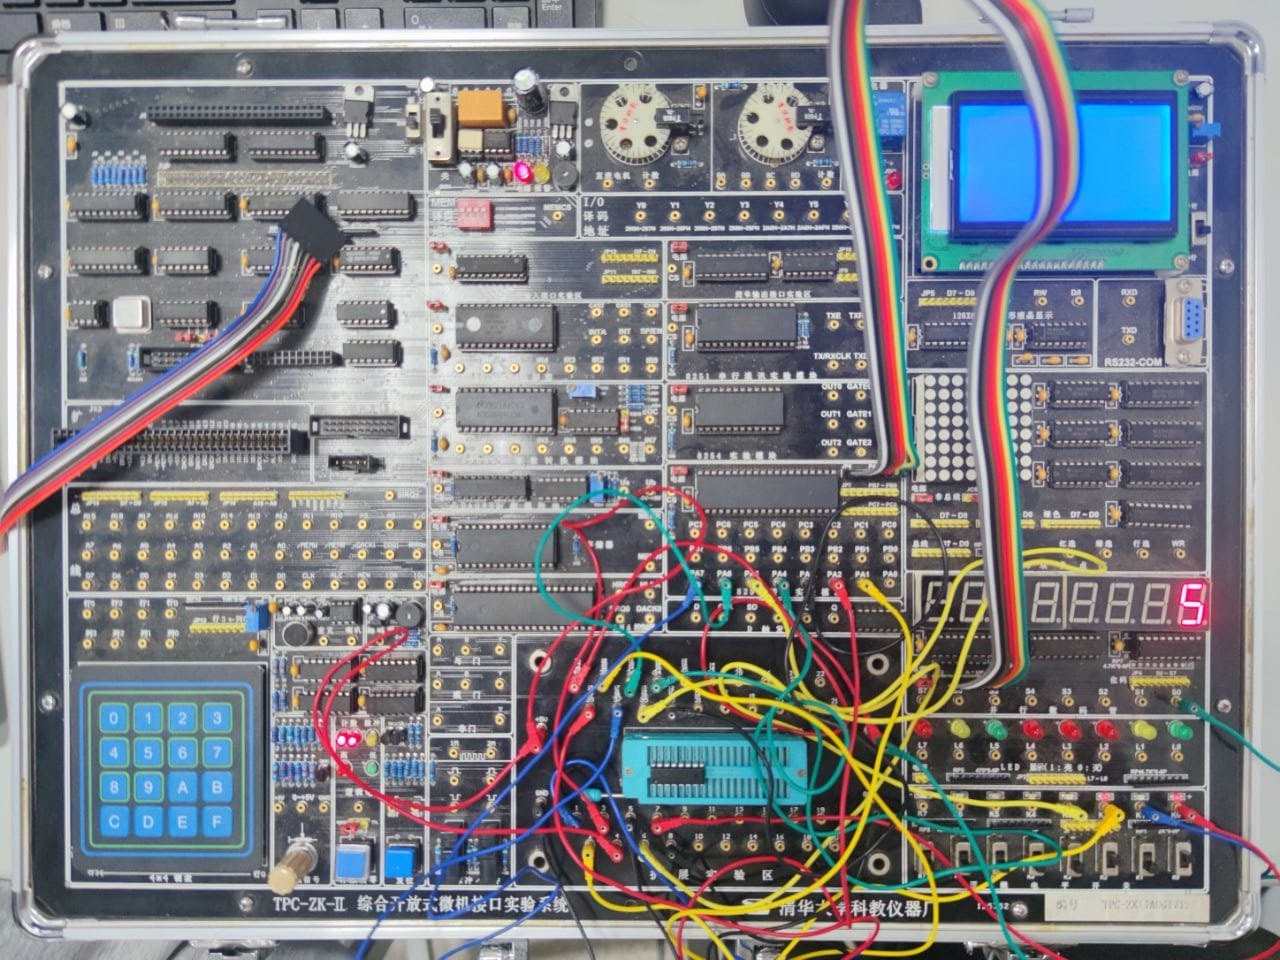
\includegraphics[width=.45\linewidth]{fig/74LS237_real.jpg}
        \caption{8 位数据/地址锁存器(8D 触发器)器特性实验真实连线图}
      \end{figure}

      \begin{analyze}{8 位数据/地址锁存器(8D 触发器)器特性实验}{}
        实验结果即完成了一个锁存的效果,只有在下降沿的过程状态会“刷新”.
      \end{analyze}


    \subsection{双8 位数据/地址锁存器(8D 触发器)特性实验($8\times 8$ 点阵)}
    \begin{note}{接线}{}
      排线1 一端接逻辑开关输入JP1(K7-K0),一端接总线插座(D7-D0)作为触发器输入;
WR 接低电平,行选接脉冲1;红选接脉冲2.
    \end{note}
    
    \begin{figure}[htbp]
      \centering
      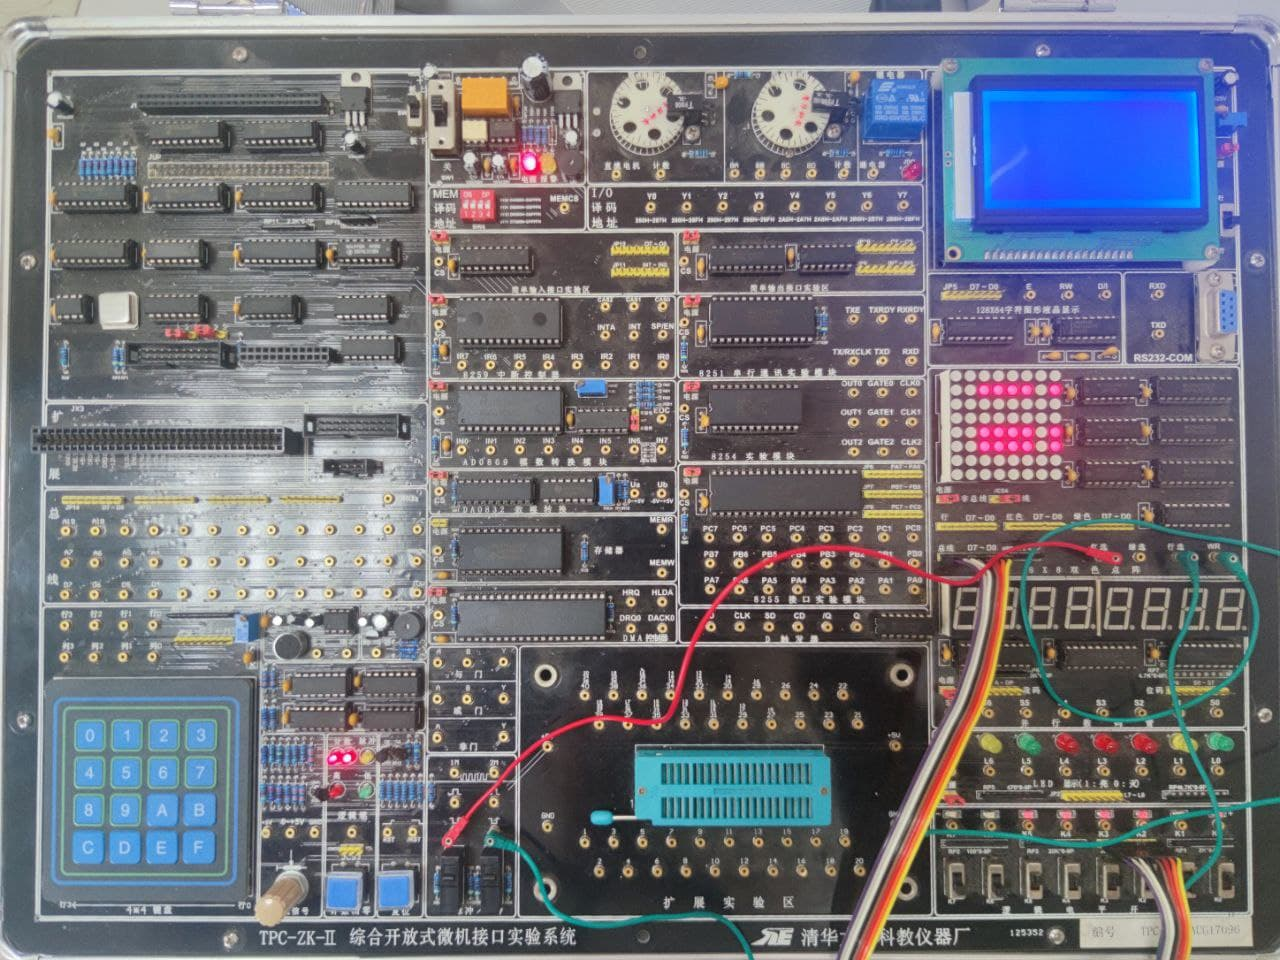
\includegraphics[width=.45\linewidth]{fig/8x8_real.jpg}
      \caption{双8 位数据/地址锁存器(8D 触发器)器特性实验真实连线图}
    \end{figure}


    \begin{analyze}{8 位数据/地址锁存器(8D 触发器)器特性实验}{}
      与上一个实验类似,存在一个锁存的效果,只有在下降沿的过程状态会“刷新”,得到的效果是比较好的,可以做到分别行选列选.
    \end{analyze}


    \subsection{扩展CD4518 计数器(双BCD 加计数器)应用}

    \begin{note}{接线}{}
      在实验箱扩展实验区顶头插入CD4518 芯片,引脚Pin16-Vcc(+5V),Pin8-GND;引
脚Pin(6-3) Q4A-Q1A 顺序接指示灯L3-L0;引脚Pin(14-11)Q4B-Q1B 顺序接指示灯L7-L4);
引脚Pin(2) Enable A 和Pin(10)ENABLE B 接高电平;Pin(1)Clock A 和Pin(9)Clock B
分别连接按键脉冲;如图~\ref{fig:CD4518_}. 
    \end{note}
    通过合理设计组合逻辑reset 信号即clock 信号,可以方便地
实现不同计数的计数器(8-4-2-1)输出,如双BCD,24 进制(时计数),60 进制(分、秒
计数). 

    由真值表可知,CD4518 可以利用clk 上升沿计数(Enable 接高电平),也可以利用enable
下降沿计数(clk 接低电平);进位可以通过各位输出状态用组合逻辑产生,也可利用输出
状态Q4 作为进位接十位Enable B. 

    \begin{figure}[htbp]
      \centering
      \subfloat[一位十进制计数器]{
        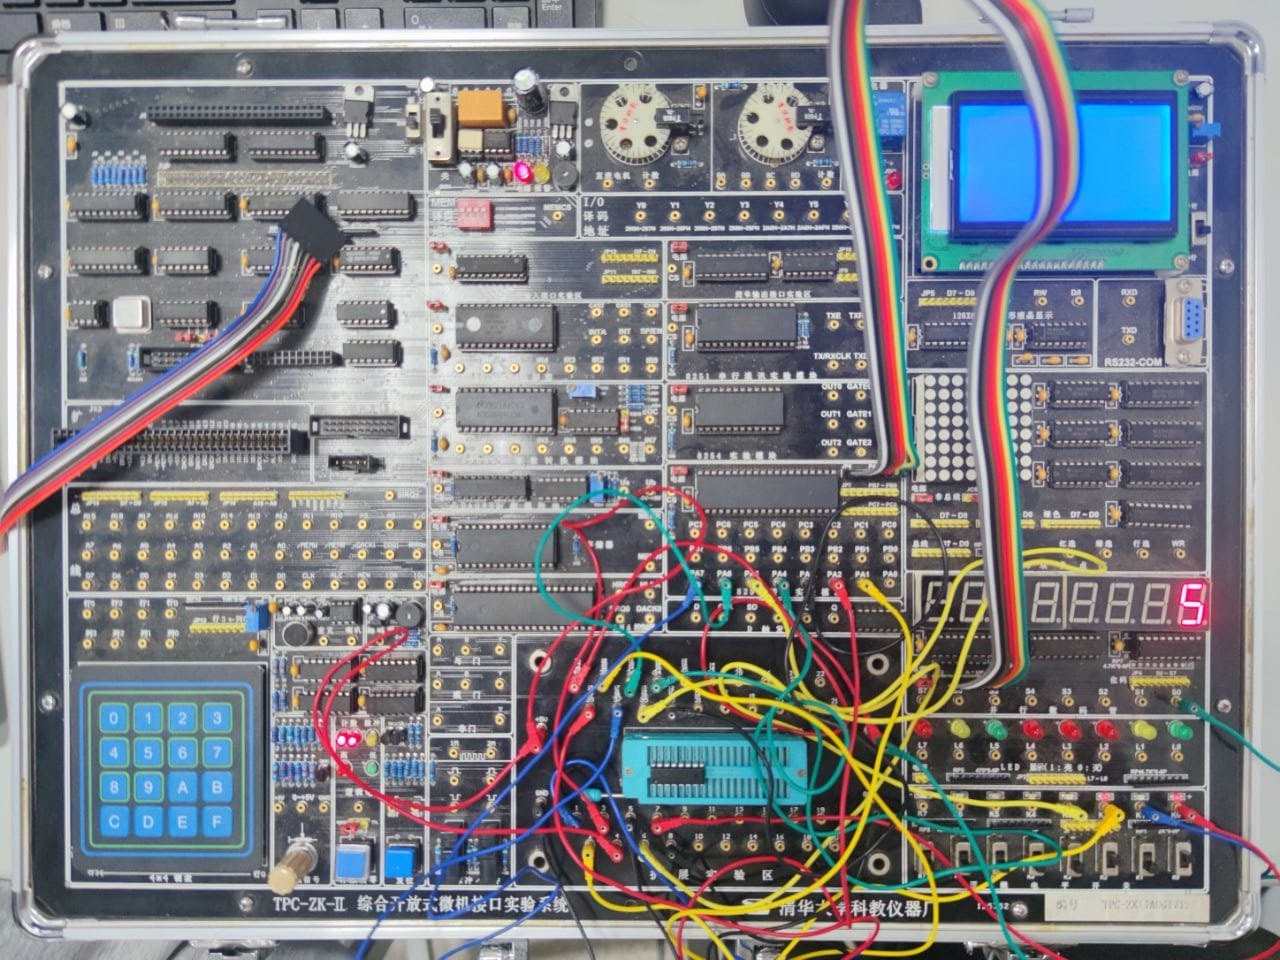
\includegraphics[width=.45\linewidth]{fig/bcd1.jpg}
        \label{subfig:bcd1}
      }\quad
      \subfloat[两位十进制计数器]{
        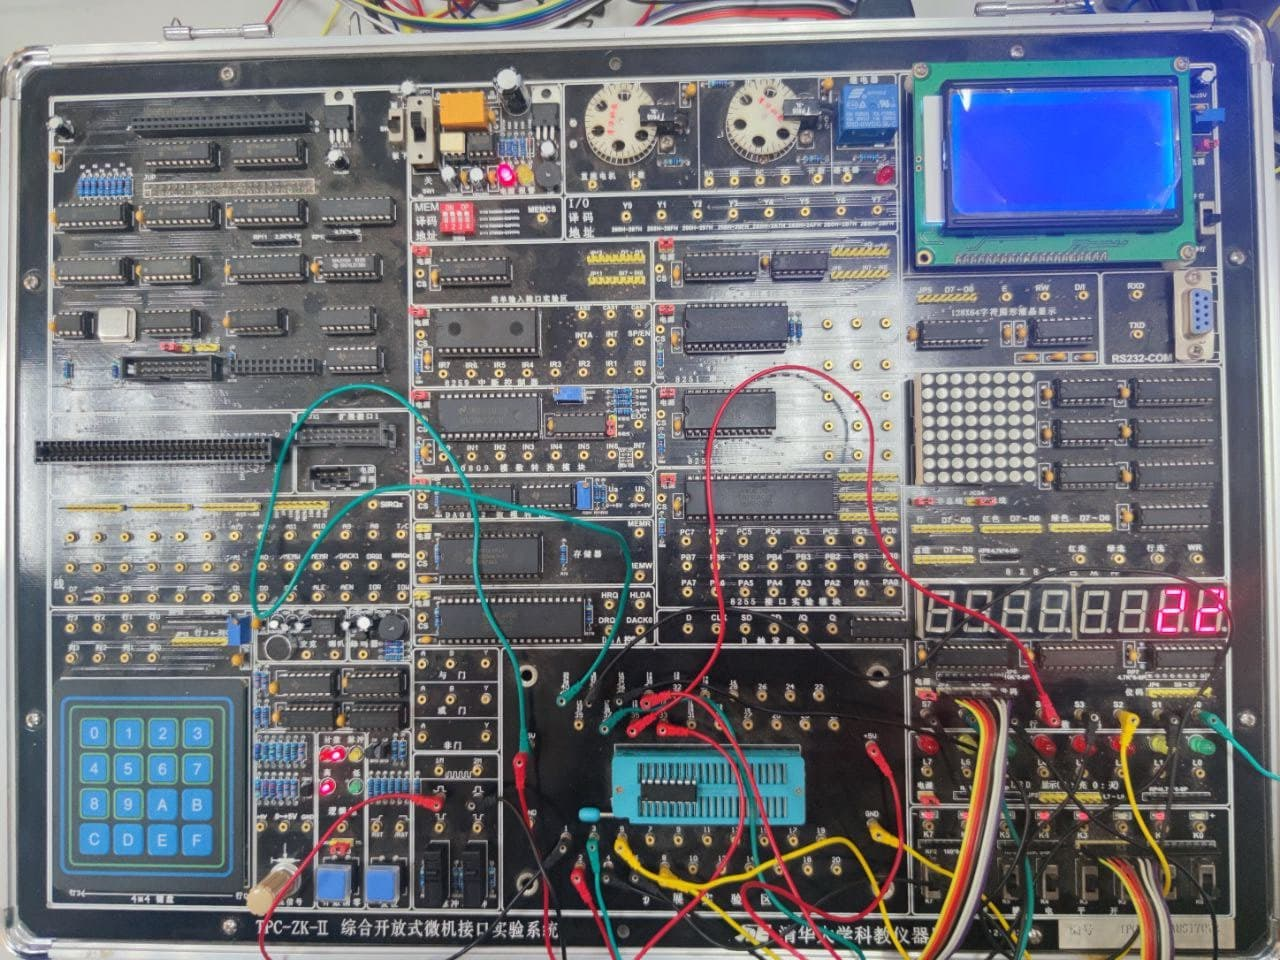
\includegraphics[width=.45\linewidth]{fig/bcd2.jpg}
        \label{subfig:bcd2}
      }
      \caption{扩展CD4518 计数器(双BCD 加计数器)应用}
    \end{figure}

    \begin{analyze}{}{}
      一位十进制计数器和双独立的 BCD 显示都成功了,
      而0-99 BCD 连接经过助教确认连接没有错误,
    \end{analyze}

    \begin{idea}{24 进制或60 进制方案}{}
      秒信号发生器由CD4060和CD4013组成,产生频率为1Hz的和时间基准信号. CD4060是14级二进制计数器/分频器/振荡器. 它与外接电阻、电容、石英晶振共同组成32768Hz振荡器,并进行14级二分频,再外加一级D触发器(CD4013)二分频,输出1Hz的时基秒信号. 秒、分、时计数器电路均采用双BCD同步加计数器CD4518计数输出BCD码,通过CD4511将BCD码显示出对应的数字,秒、分计数器是60进制计数,时是24进制计数. 时、分、秒的显示电路完全相同,均使用CD4511译码驱动数码管. 秒校时采用等待校时法,正常工作时,开关S3拨到“走时”,进行对秒信号校对,将S3拨到“停”,待标准时间一到,立即拨到“走时”位置,恢复正常走时. 分和时通过开关直接输入脉冲信号校准,每按一次开关,加一次数.  

60进制电路工作原理:当时间是60秒的时候,4518的十位输出的BCD码是0110,通过一个与门电路(CD4581)接在4518的Q2B和Q3B端,当到60秒时,这两端同时输出1,通过与门电路输出1给CD4518清零,数字从00开始重新计数,同时给分信号或者时信号来一个脉冲加1.  

24进制电路工作原理同60进制电路类似,只不过取的信号是24. 4518输出的BCD码是0010 0100,取4518的Q2B和Q3A端即可.  

\begin{center}
  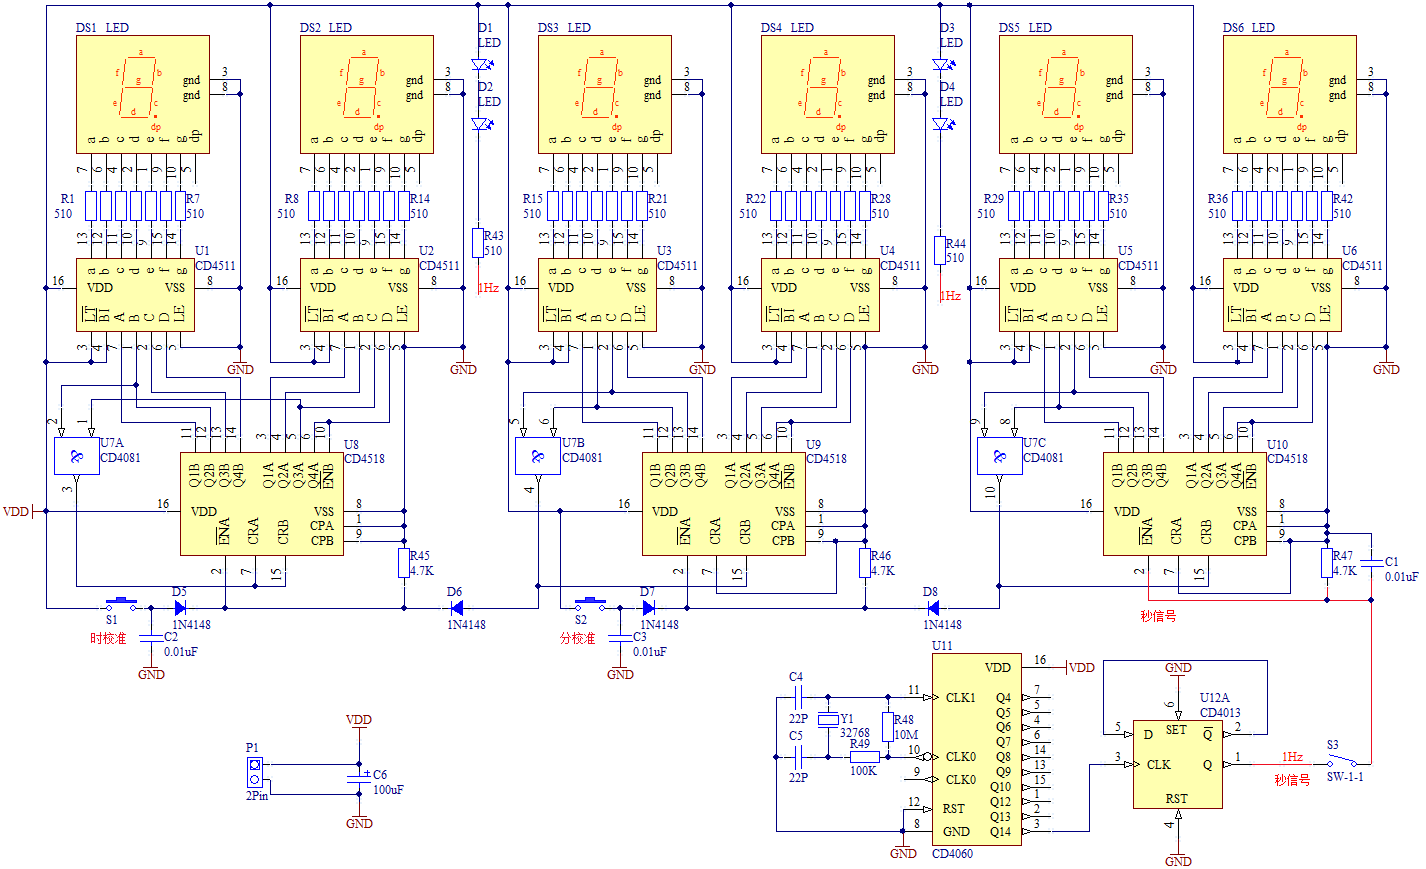
\includegraphics[width=.8\linewidth]{fig/counter_clock.png}
  \captionof{figure}{24 进制或60 进制方案电路图}
\end{center}
  

\begin{idea}{总结}{}
  总结一下,主要的区别就是“如何进位”,十进制进位使用 BCD码的进位信号即可,
  而在 24 和 60 进制中则需要\textbf{通过逻辑表达式给出进位的信号},操作过程即是:
  24进制取4518的Q2B和Q3A端,60进制4518的Q2B和Q3B端. 
\end{idea}

电路没有断电记忆时间功能,断电后需要重新校时.  
      \footnote{参考 \url{http://www.diyleyuan.com/JC/162.html}.}
    \end{idea}

  \subsection{CAD 逻辑设计与仿真}

    \subsubsection{基本触发器模块}

    编写了基本的触发器模块,分别使用\texttt{always}“\texttt{=}”和“\texttt{<=}”赋值语句,实现变量的复
    制(获取),其识时序逻辑HDL 阻塞(Blocking)与非阻塞(Nonblocking) 赋值语句.

    其 Verilog 代码在下方,其区别仅在赋值方式的一行.
    
    \newpage
    \begin{multicols}{2}
      \begin{lstlisting}[language=verilog, title=Blocking, numbers=none]
module dff #(parameter DELAY = 0)(
  input d,
  input clk,
  output q,
  output w
  );
  reg q, w;
  always @(posedge clk)
  begin
    w = #DELAY d;
    q = w; // blocking
  end
endmodule
      \end{lstlisting}
      \begin{lstlisting}[language=verilog, title=Nonblocking, numbers=none]
module dff #(parameter DELAY = 0)(
  input d,
  input clk,
  output q,
  output w
  );
  reg q, w;
  always @(posedge clk)
  begin
    w <= #DELAY d;
    q <= w; // nonblocking
  end
endmodule
      \end{lstlisting}
    \end{multicols}

    \begin{analyze}{基本触发器模块}{}
      分别运行上述两种代码,可以得到阻塞赋值的RTL级电路图~\ref{fig:vivado:blocking}~和非阻塞赋值的RTL级电路图~\ref{fig:vivado:nonblocking}.
      可以观察到,非阻塞赋值需要使用额外的寄存器以实现并行处理,
      在原理上是比较好理解的.
    \end{analyze}

    \begin{figure}[htbp]
      \centering
      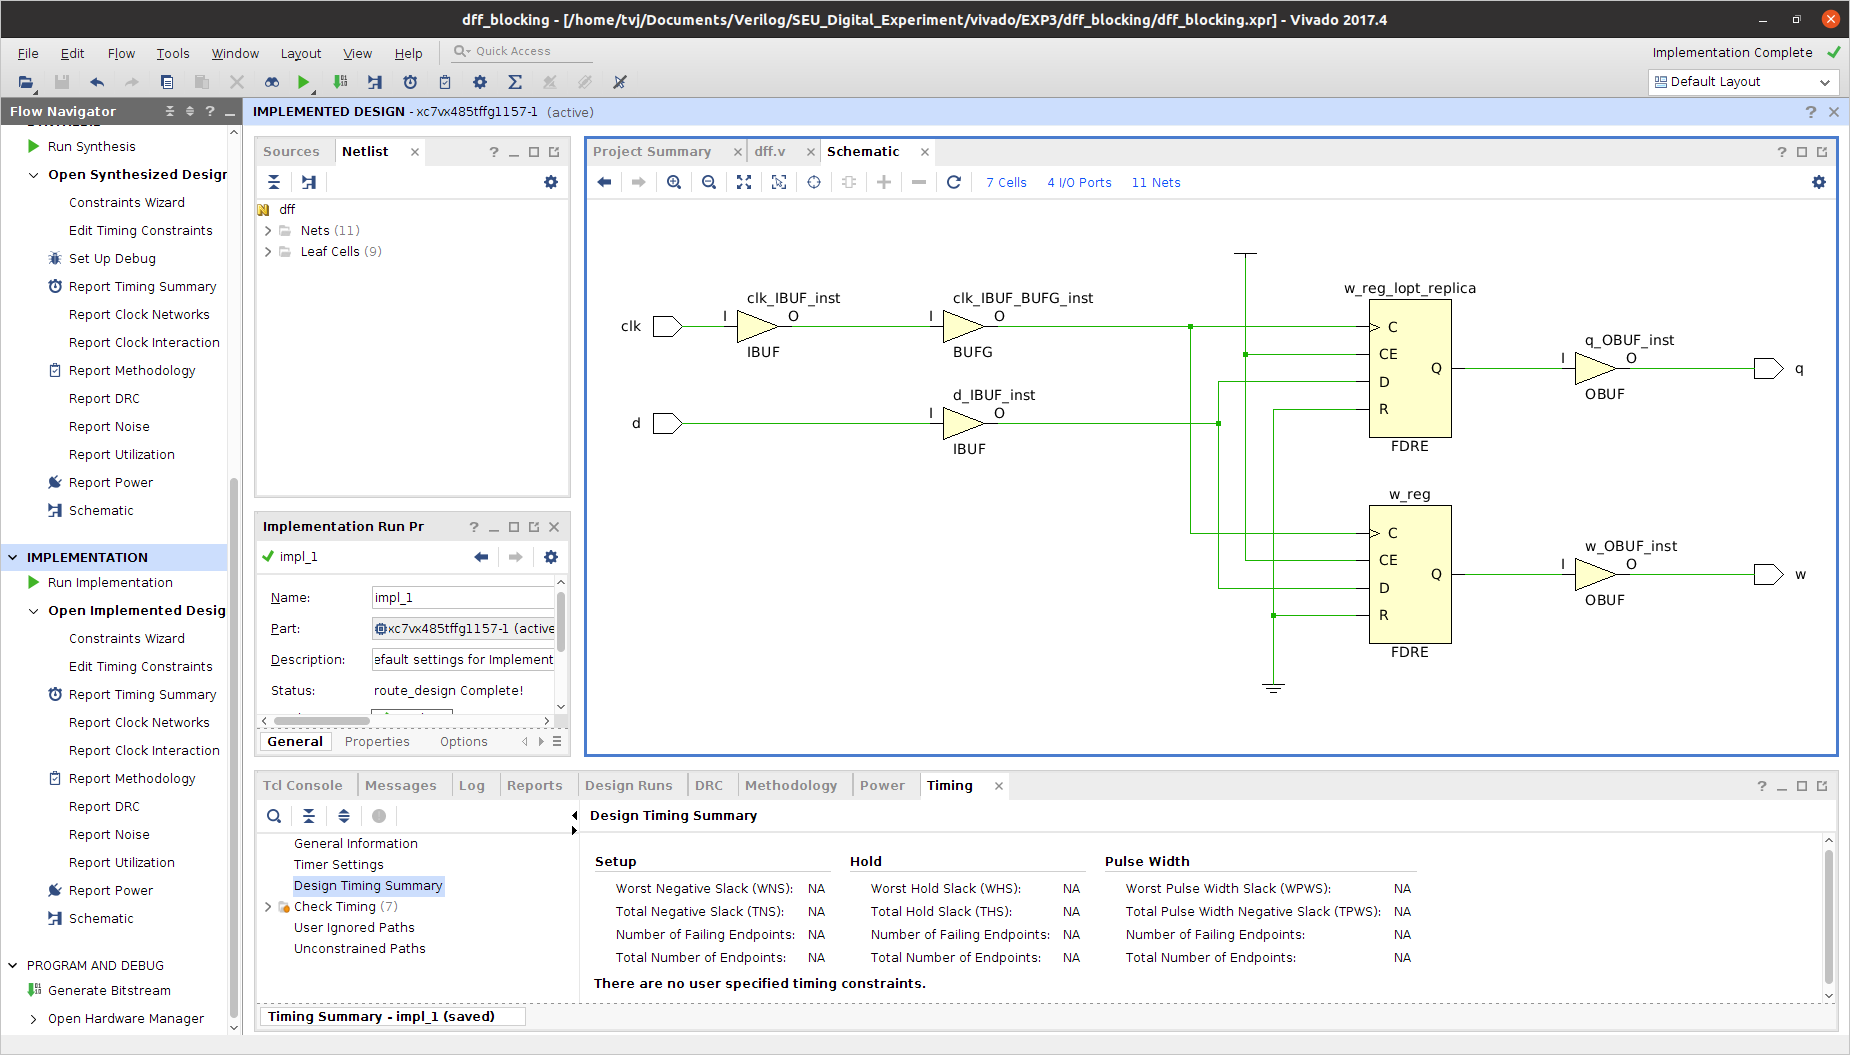
\includegraphics[width=\linewidth]{fig/vivado/dff_blocking.png}
      \caption{阻塞赋值的电路}
      \label{fig:vivado:blocking}
    \end{figure}
    \begin{figure}[htbp]
      \centering
      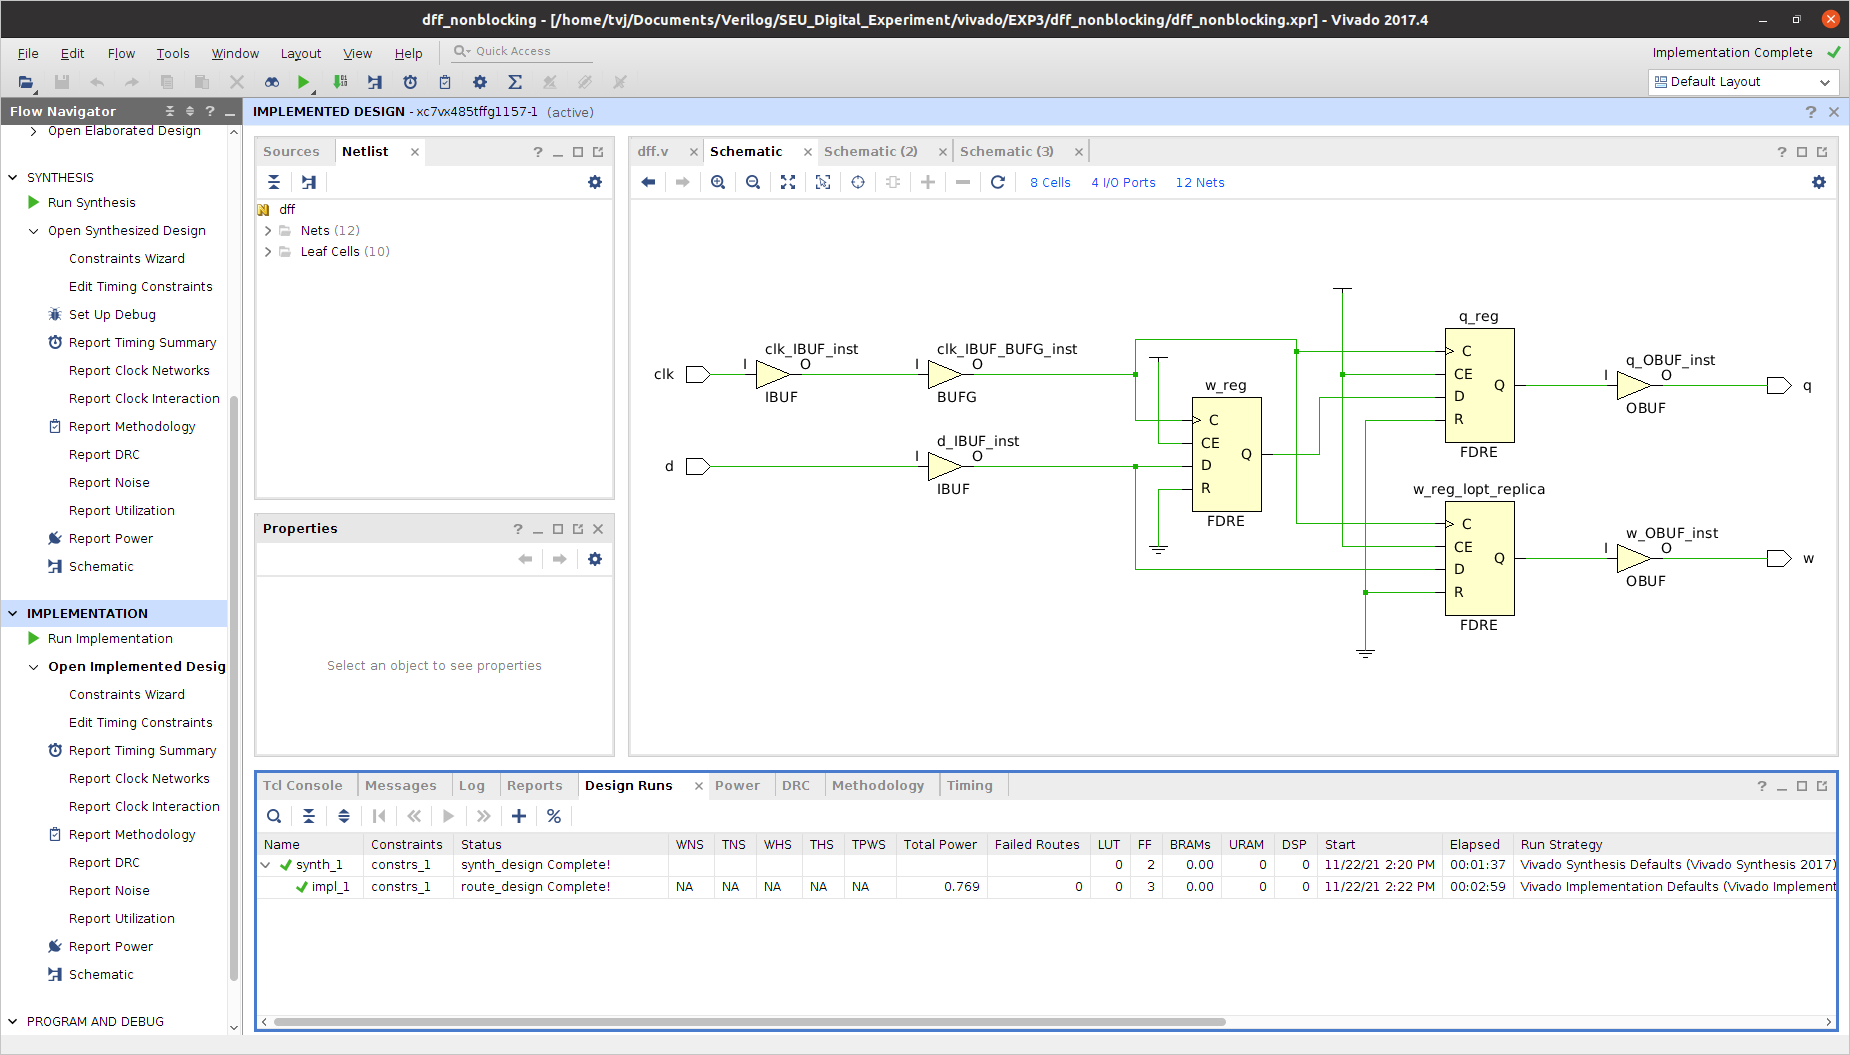
\includegraphics[width=\linewidth]{fig/vivado/dff_nonblocking.png}
      \caption{非阻塞赋值的电路}
      \label{fig:vivado:nonblocking}
    \end{figure}

    \subsubsection{74LS273模块}
      74LS273 等效功能模块Verilog HDL 如下:
          \begin{lstlisting}[language=verilog, title=74LS273, numbers=none]
module ff273v (din, clk, clr, dout);
  input [7:0] din;
  input clk, clr;
  output [7:0] dout;
  reg [7:0] dout;
  reg [7:0] dinn,dins;
  always @(posedge clk or negedge clr)
  begin
  if (!clr)
    dout <= 8'b00000000;
  else
    begin
      dout<=din;
    end
  end
endmodule
      \end{lstlisting}

      \begin{figure}[htbp]
        \centering
        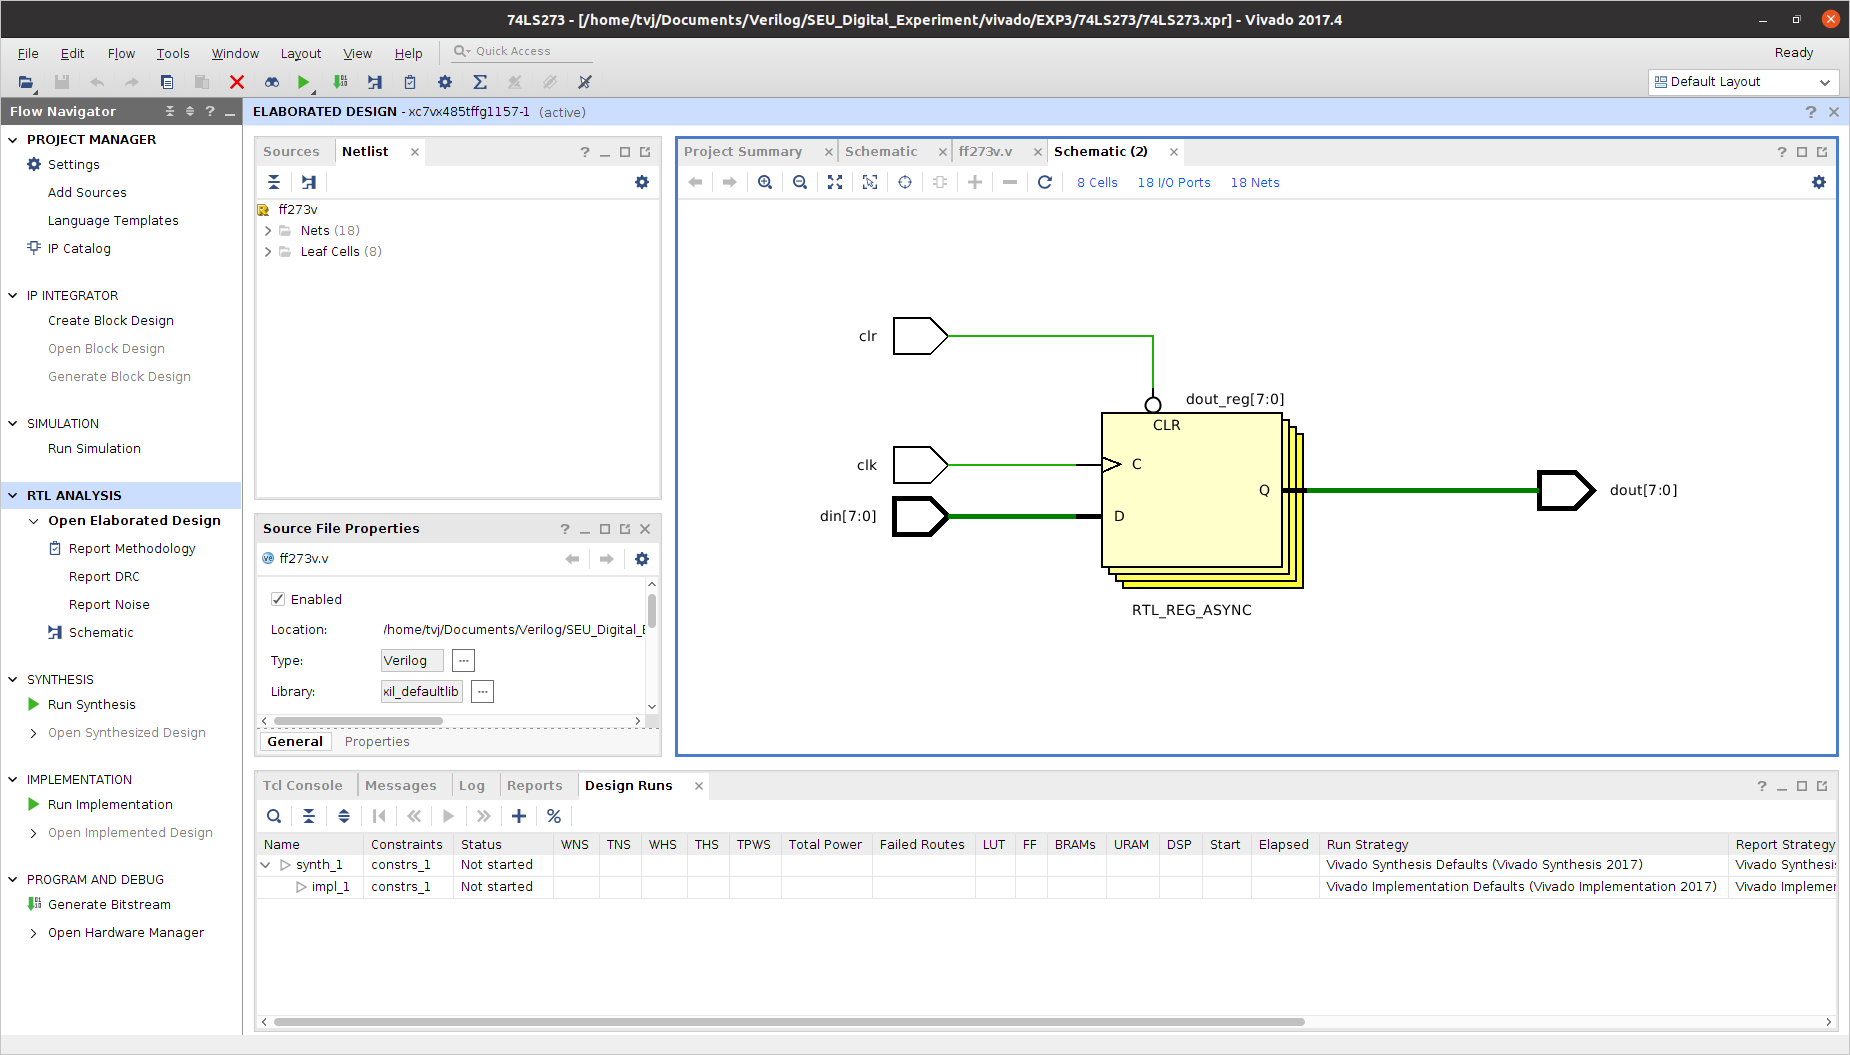
\includegraphics[width=\linewidth]{fig/vivado/ff273v_RTL.png}
        \caption{ff273v RTL电路}
      \end{figure}
      \begin{figure}[htbp]
        \centering
        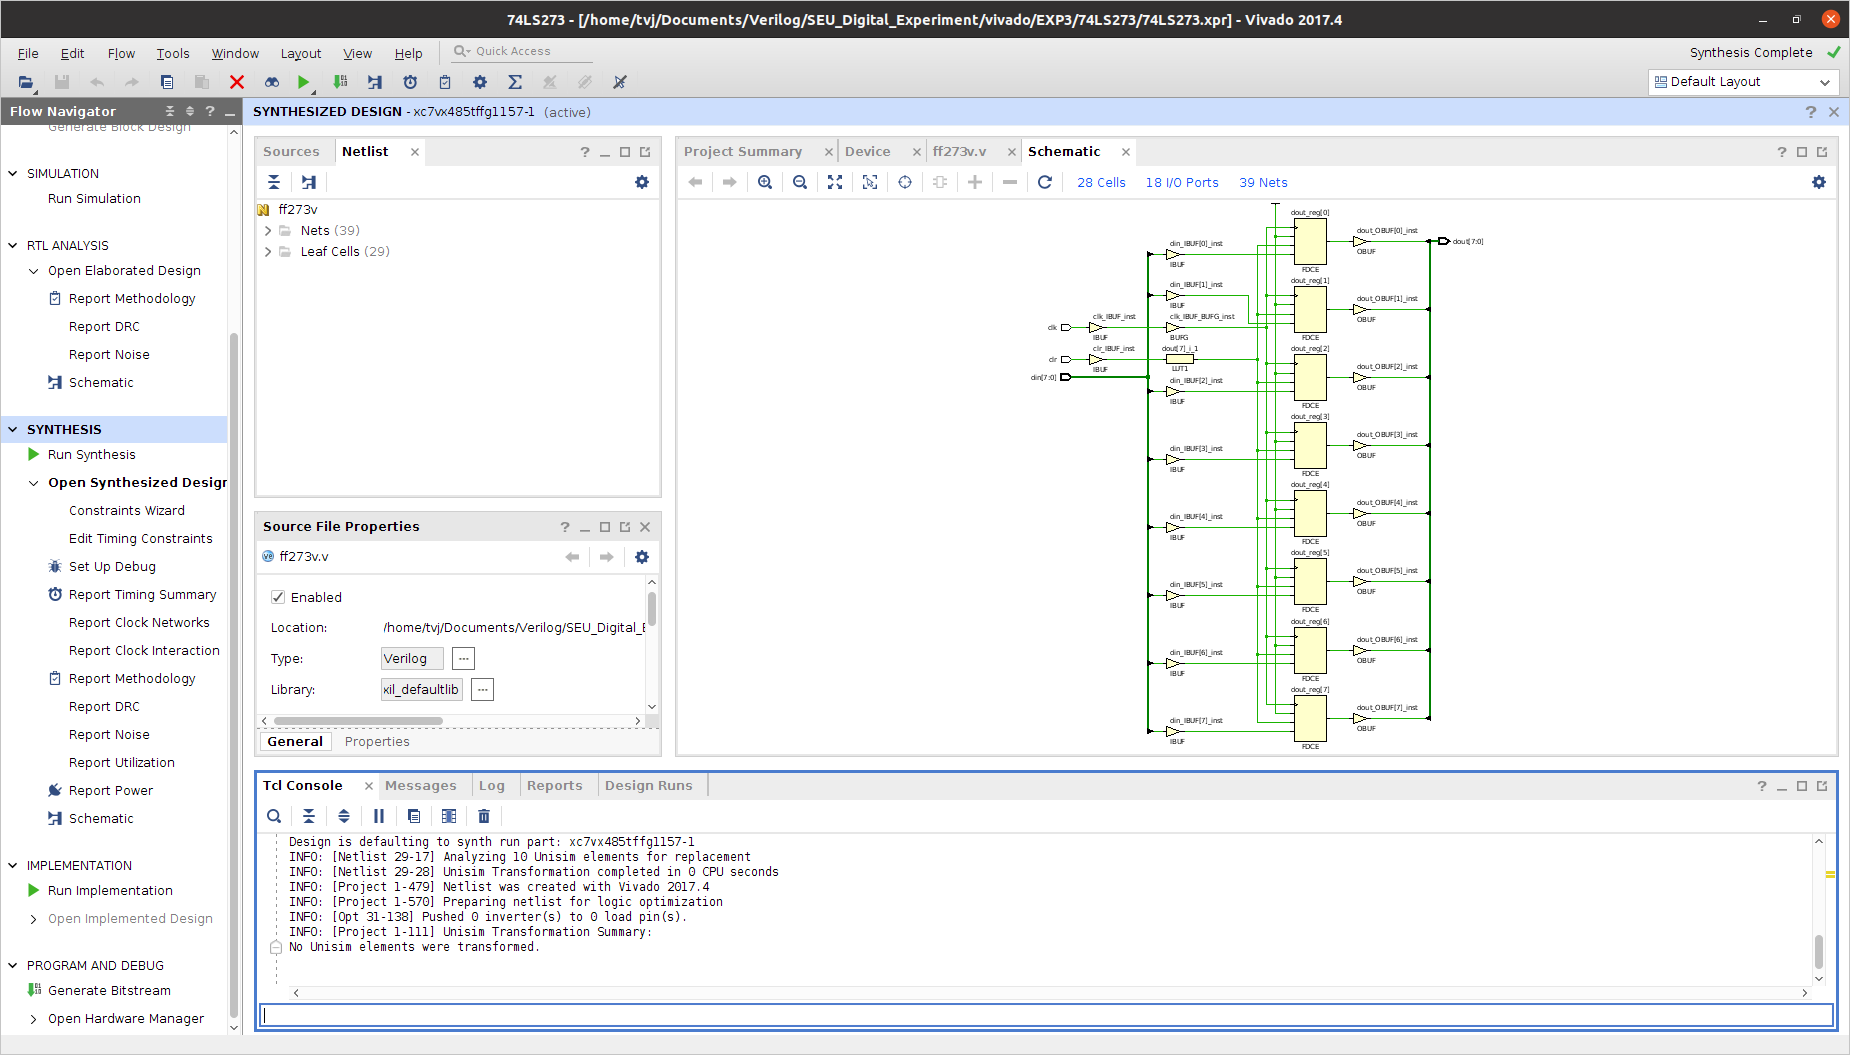
\includegraphics[width=\linewidth]{fig/vivado/ff273v_synthesis.png}
        \caption{ff273v Synthesis 电路}
        \label{fig:ff273v_synthesis}
      \end{figure}
      \begin{figure}[htbp]
        \centering
        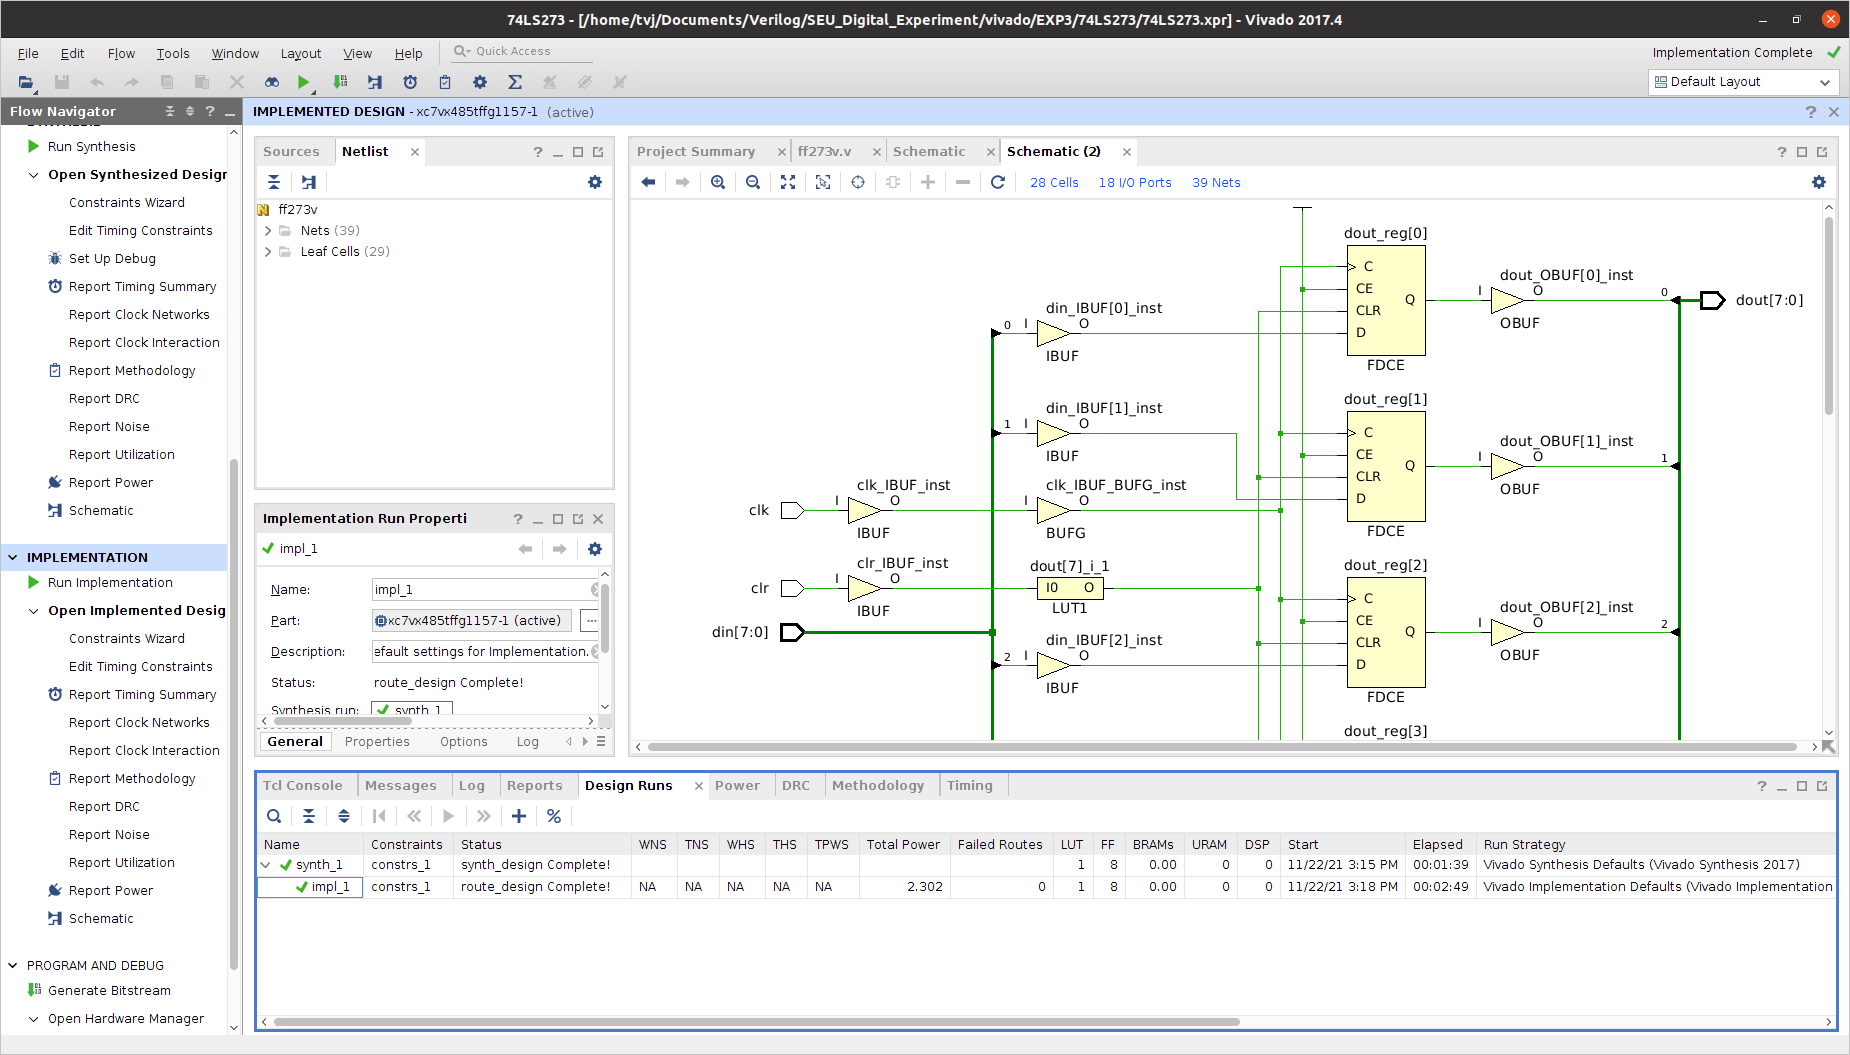
\includegraphics[width=\linewidth]{fig/vivado/ff273v_implementation.png}
        \caption{ff273v Implementation 电路}
        \label{fig:ff273v_implementation}
      \end{figure}

      \begin{analyze}{}{}
        Synthesis(图~\ref{fig:ff273v_synthesis})和Implementation(图~\ref{fig:ff273v_implementation})实际上是一样的,有可能是和选择的 device 有关.
        不过对于其整体的结构已经有了较为深入的了解了.
        从图中可以较为清楚地看出8位锁存的方式.
      \end{analyze}

      \newpage
      \subsubsection{Cnt10 定时计数器}


      \begin{multicols}{2}
        \begin{lstlisting}[language=verilog, title=fre\_ctrl.v, numbers=none]
module fre_ctrl (clk_in2,clk2);
  input clk_in2;
  output clk2;
  reg clk;
  reg [31:0] k;
  reg a, b, c;
  always @(negedge clk_in2)
  begin
  if (k >= 10000000)
    begin
      clk <= ~clk2; // clock signal
      a <= ~clk2;
      b = a ^ clk;
      c = a & clk;
      k <= 0;
    end
  else
    k <= k + 1;
  end
endmodule
        \end{lstlisting}
        \begin{lstlisting}[language=verilog, title=count10.v, numbers=none]
module count10 (clk, clr, qout, c);
  input clk, clr;
  output [3:0] qout;
  output c;
  reg [3:0] qout;
  reg c;
  always @(posedge clk or posedge clr)
  if (clr)
    qout <= 0;
  else
    begin
      if (qout>=9)
        begin
          qout<=0;
          c<=1;
        end
      else
        begin
          qout <= qout + 1;
          c <= 0;
        end
      end
    end /* This 'end' is missing in Ref. [1] */
  end
endmodule
        \end{lstlisting}
        \begin{lstlisting}[language=verilog, title=disp.v, numbers=none]
module disp (qout,clk,led1);
  input [3:0] qout;
  input clk;
  output [6:0] led1;
  reg [6:0] led1;
  always @(posedge clk)
  begin
    case(qout)
    0: led1 = 7'b0000001;
    1: led1 = 7'b1001111;
    2: led1 = 7'b0010010;
    3: led1 = 7'b0000110;
    4: led1 = 7'b1001100;
    5: led1 = 7'b0100100;
    6: led1 = 7'b0100000;
    7: led1 = 7'b0001111;
    8: led1 = 7'b0000000;
    9: led1 = 7'b0000100;
    default: led1 = 7'b0000001;
    endcase
  end
endmodule /* This is missing in Ref. [1] */
        \end{lstlisting}
      \end{multicols}

  \section{选作探索与应用设计}

    \subsection{74LS161 可加载4 位二进制计数电路}

    \begin{lstlisting}[language=verilog, title=My74LS161]
module My74LS161(
  input wire CR, LD, CTP, CTT, CP,
  input wire [3:0] D,
  output reg Co,
  output reg [3:0] Q
  );

  always @ (posedge CP or negedge CR) begin
    if ( !CR ) Q = 4'b0;  // Asynchronous clear takes the highest priority
    else if ( !LD ) Q = D;
    else if ( CTP && CTT ) Q = Q + 4'b1;
    if ( Q == 4'b1111 ) Co = 1;
  else Co = 0;
  end
endmodule
    \end{lstlisting}

    学习了网上的代码\footnote{代码:\url{https://github.com/Teddy-van-Jerry/LCDF_Expr/blob/master/Expr13/Report13.md}.},大致了解了整体的架构方式.

    \subsection{24 和 60 进制计数显示系统(时钟)}

    

    \begin{lstlisting}[language=verilog, title=TOP.v]
module top_rtc(input rst, clk, output[6:0] S_L, S_M, M_L, M_M, H_L, H_M);
  wire[3:0] w1, w2, w3, w4, w5, w6;
  segment_7 s1(.bcd(w1), .y(S_L));
  segment_7 s2(.bcd(w2), .y(S_M));
  segment_7 s3(.bcd(w3), .y(M_L));
  segment_7 s4(.bcd(w4), .y(M_M));
  segment_7 s5(.bcd(w5), .y(H_L));
  segment_7 s6(.bcd(w6), .y(H_M));
  rtc c1(.clk(clk), .rst(rst), .sl(w1), .sm(w2), .ml(w3), .mm(w4), .hl(w5), .hm(w6));
endmodule
    \end{lstlisting}

        \begin{lstlisting}[language=verilog, title=BCD\_SEVEN\_SEGMENT.v]
module segment_7(input [3:0]bcd, output reg [6:0]y);
  always @(*)
  case(bcd)
    4'd0: y = 7'b1111_110;
    4'd1: y = 7'b0110_000;
    4'd2: y = 7'b1101_101;
    4'd3: y = 7'b1111_001;
    4'd4: y = 7'b0110_011;
    4'd5: y = 7'b1011_011;
    4'd6: y = 7'b1011_111;
    4'd7: y = 7'b1110_000;
    4'd8: y = 7'b1111_111;
    4'd9: y = 7'b1111_011;
  endcase
endmodule
    \end{lstlisting}

    
        \begin{lstlisting}[language=verilog, title=COUNTER.v]
module rtc(input rst,clk, output [3:0] sl,sm,ml,mm,hl,hm );
  reg [3:0] sl0,sm0,ml0,mm0,hl0,hm0;
  wire clk_1sec;
  assign sl=sl0;
  assign sm=sm0;
  assign ml=ml0;
  assign mm=mm0;
  assign hl=hl0;
  assign hm=hm0;
  assign clk_1sec=clk;//let clk_1sec is drived by 1sec time period clock
  always@(posedge clk)
    if(rst) begin
      sl0<=0;
      sm0<=0;
      ml0<=0;
      mm0<=0;
      hl0<=0;
      hm0<=0;
    end
  else if(sl0<9) begin
    if(clk_1sec)
    sl0<=sl0+1;
  end
    else if(sm0<5) begin
      sm0<=sm0+1;  
      sl0<=0;
    end
  else if(ml0<9) begin
    sl0<=0;
    sm0<=0;
    ml0<=ml0+1;
  end
  else if(mm0<5) begin
    sl0<=0;
    sm0<=0;
    ml0<=0;
    mm0<=mm0+1;  
  end
  else if(((hm0<2) && (hl0<9))||((hm0==2)&&(hl0<3))) begin
    sl0<=0;
    sm0<=0;
    ml0<=0;
    mm0<=0;
    hl0<=hl0+1;
  end
  else if(hm0<2)
    begin
    sl0<=0;
    sm0<=0;
    ml0<=0;
    mm0<=0;
    hl0<=0;
    hm0<=hm0+1; 
    end
  else if((hm0==2)&&(hl0==3)&&(mm0==5)&&(ml0==9)&&(sm0==5)&&(sl0==9)) begin
    sl0<=0;
    sm0<=0;
    ml0<=0;
    mm0<=0;
    hl0<=0;
    hm0<=0;
  end
endmodule
    \end{lstlisting}
    
    \begin{lstlisting}[language=verilog, title=SIM.v]
module tb(); // testbench
  wire [6:0] sl,sm,ml,mm,hl,hm;
  reg clk;
  reg rst;
  
  always #1 clk=~clk; // clock signal
  
  top_rtc r0(rst,clk,sl,sm,ml,mm,hl,hm);
  
  initial begin
    clk=0;
    rst=0;
    #5;
    rst=1;
    #5;
    rst=0;
    #4500 $finish();
  end
  initial begin
    $dumpvars();
    $dumpfile("dump.vcd");
   
    $monitor($time, "rst= %b,SEC_L= %b, SEC_M= %b, MIN_L= %b, MIN_M= %b, H_L= %b, H_M= %b", rst, sl, sm, sl, mm, hl, hm);

  end
endmodule
    \end{lstlisting}

    \begin{analyze}{24 和 60 进制计数显示系统(时钟)}{}
      学习了网上的代码\footnote{代码地址:\url{https://github.com/T-V-J/24-12_DIGITAL_CLOCK_DESIGN_USING_VERILOG},这是我 fork 后的项目.},
      了解了其整体的结构和具体方法.
       
      其中几个重要的模块就是计数器(\texttt{COUNTER.v})和 BCD 七段管显示(\texttt{BCD\_SEVEN\_SEGMENT.v}),这些在之前的研究中已经较为清楚了,此处不加赘述.
      此处最重要的是较为完整的\texttt{层次性},这里的 \texttt{TOP.v} 即是做了整合的工作,将计数和现实整合在一个完整的大项目中了,调用了计数器和显示.
      而 \texttt{SIM.v} 通过已有接口增加了时钟信号.
    \end{analyze}

    \newpage
    \begin{figure}[htbp]
      \centering
      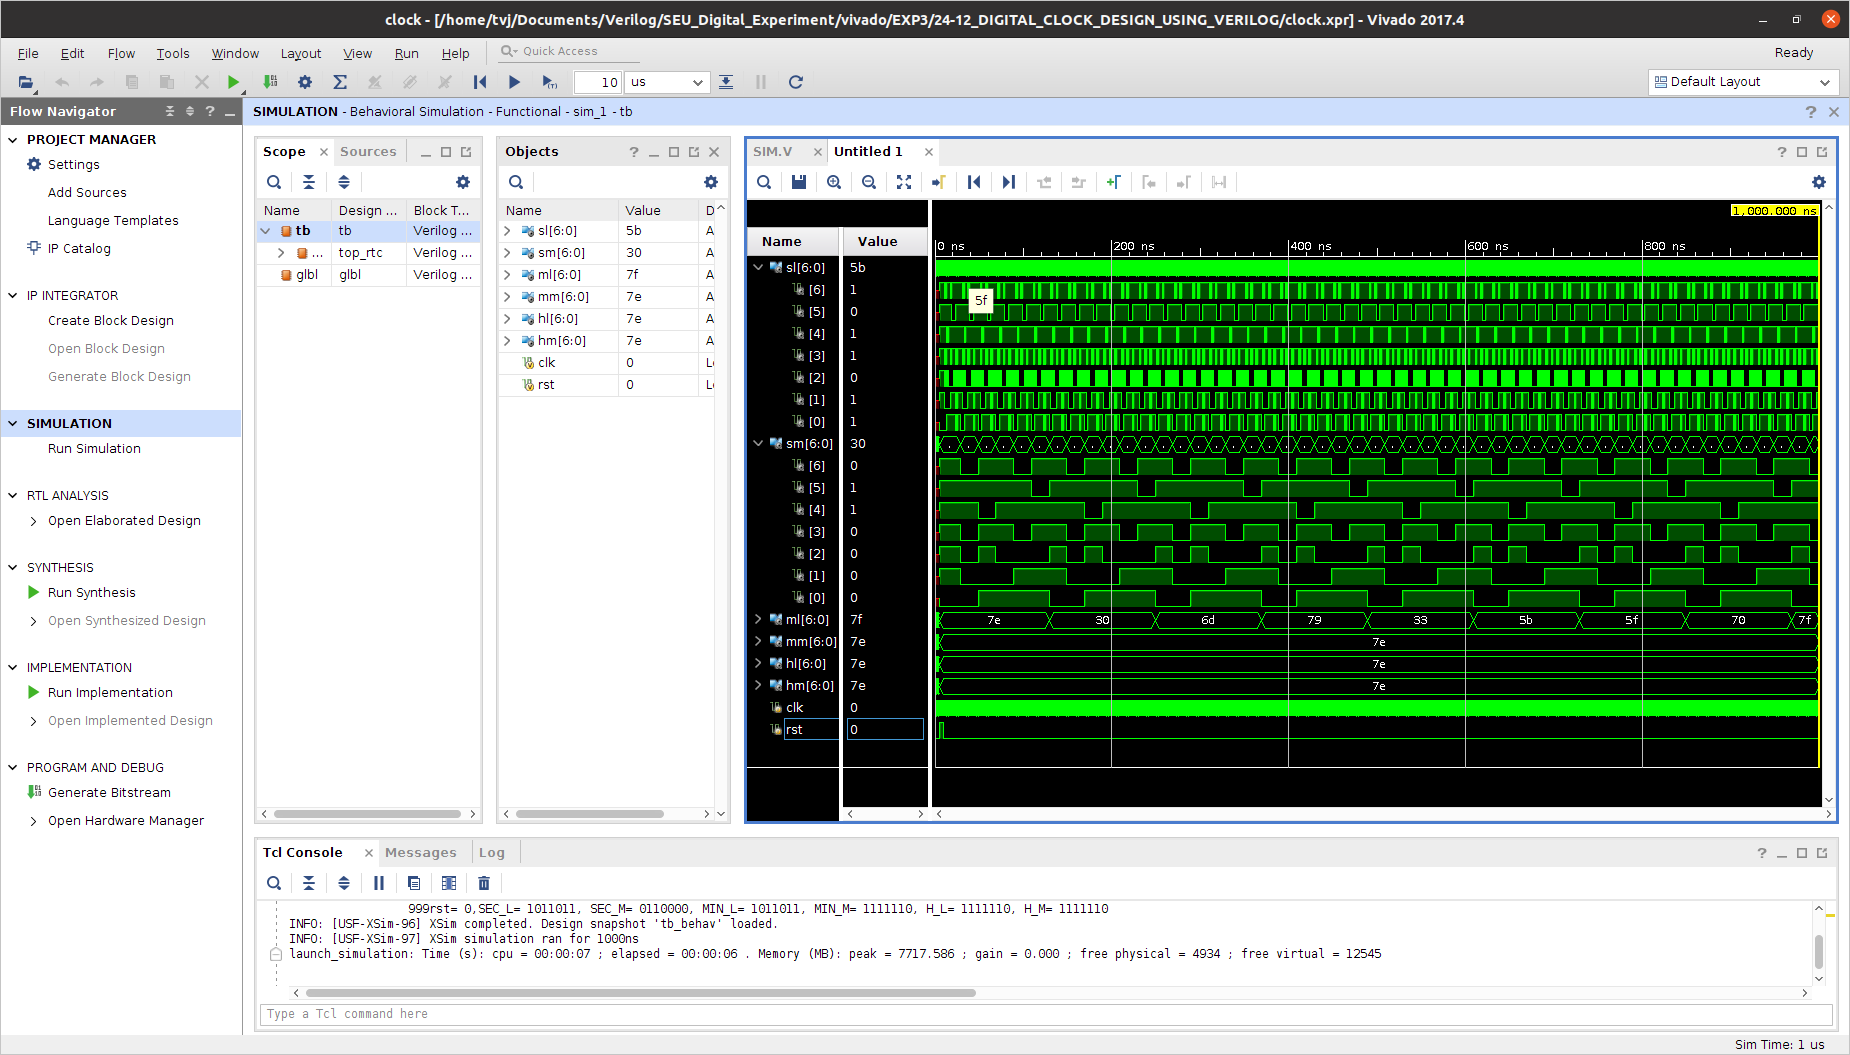
\includegraphics[width=\linewidth]{fig/vivado/24_60_simu.png}
      \caption{24 和 60 进制计数显示系统(时钟)行为仿真结果\protect\footnotemark}
      \label{fig:20_60_simu}
    \end{figure}
    \footnotetext{最上面一组是秒的个位,第二组是秒的十位,再往下是分的两位和时的两位.}
    \begin{figure}[h!]
      \centering
      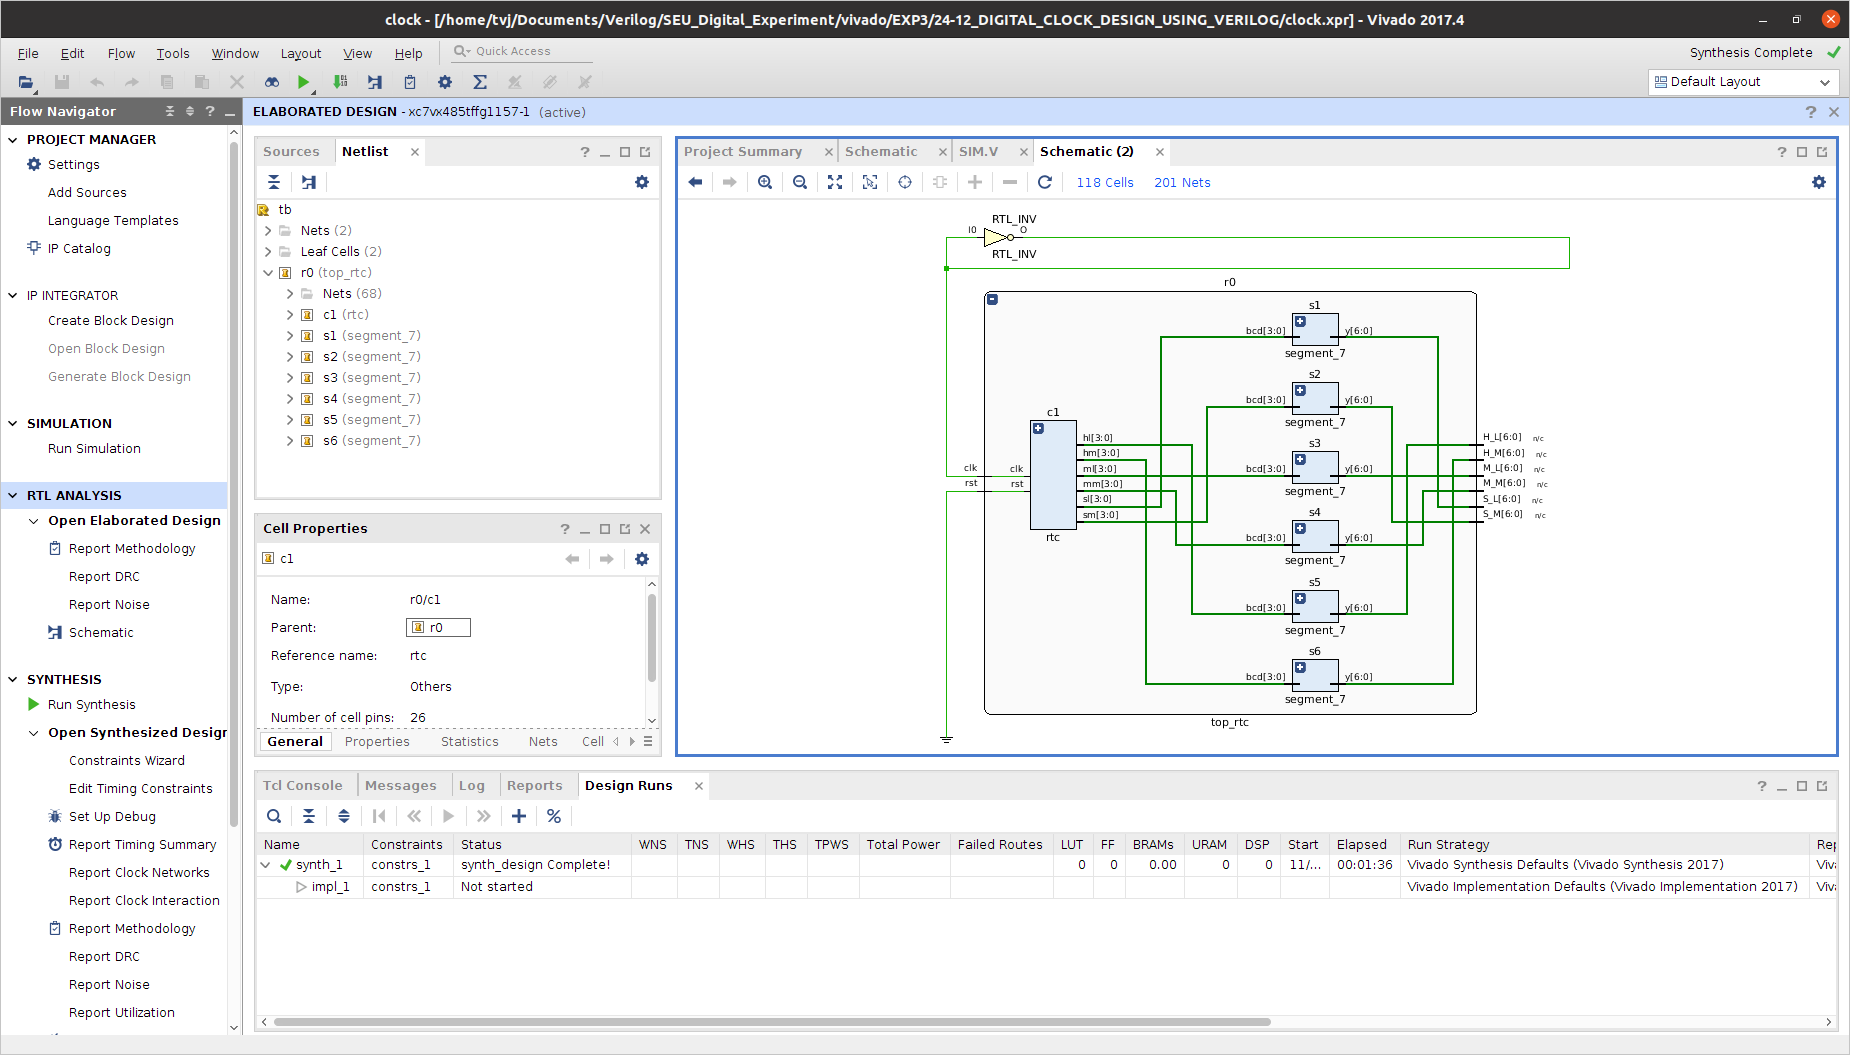
\includegraphics[width=\linewidth]{fig/vivado/24_60_RTL.png}
      \caption{24 和 60 进制计数显示系统(时钟)RTL级电路}
      \label{fig:20_60_RTL}
    \end{figure}


  \section{实验总结}

    \begin{enumerate}
      \item 需要用到实验箱的部分和 Vivado 实验关联紧密,在做硬件实验部分的时候就需要对结构和各个元件有深入的认识. 一个简单的例子就是我们在理论课上学习的锁存器、寄存器等是需要上升沿信号激活的,而这个信号在实验中即是使用开关/脉冲信号/信号源,并在实际连线操作中会遇到更多的问题. 而这个过程是非常锻炼我们的动手操作能力.
      \item Vivado 中编写程序的感觉和 C++ 中类似,都是从一个总体思路开始层层向下(至少我是这样的,不过不排除先从模块再整合的思路),有一个总体要求(Verilog 中的 testbench 或者总的 top 结构,C++ 中的 \texttt{main} 函数)向下有其他的模块(module,而在 C++ 中则是类或者函数).
      \item 其他的内容在对应的各个部分已有分析.
    \end{enumerate}

    % 打印参考文献
    \addcontentsline{toc}{section}{参考文献}
    \printbibliography[sorting=none]

    \newpage
    \addcontentsline{toc}{section}{附录 A:实验报告 \LaTeX 模板}
    \section*{附录 A:实验报告 \LaTeX 模板}

        实验报告使用自己编写的 \LaTeX 模板(\texttt{SEU-Digital-Report.cls}),
        在基本适配 Microsoft Word 版报告的格式要求之外,
        增加了更多的功能,使得报告看起来更加优雅多彩.

        后续升级后,报告模板将于 \url{https://github.com/Teddy-van-Jerry/TVJ-Digital-Report} 基于 MIT License 开源共享.

        编译需要使用 \texttt{XeLaTeX + Biber},封面页修改如下内容即可.
        \begin{lstlisting}[
          language=tex,
          morekeywords={
            expno,
            expname,
            expauthor,
            expID,
            expmates,
            expmatesID,
            expmajor,
            explab,
            expdate,
            expreportdate,
            expgrade,
            exptutor,
            today
          }
        ]
%% 使用实验报告模板类(字体大小 11pt 约为五号字)
\documentclass[11pt]{SEU-Digital-Report}

%%%%%%%%%%%%%%%%%%%% 报告基本信息 %%%%%%%%%%%%%%%%%%%%
\expno{三} % 实验序号
\expname{时序逻辑与设计} % 实验名称
\expauthor{赵舞穹} % 姓名
\expID{61520522} % 学号
\expmates{郑瑞琪} % 同组
\expmatesID{61520523} % 学号(同组)
\expmajor{工科试验班} % 专业
\explab{计算机硬件技术} % 实验室
\expdate{2021年11月12日} % 实验日期
\expreportdate{\today} % 实验日期
\expgrade{} % 成绩评定
\exptutor{冯熳} % 评阅教师
%%%%%%%%%%%%%%%%%%%%%%%%%%%%%%%%%%%%%%%%%%%%%%%%%%%%
        \end{lstlisting}

    \addcontentsline{toc}{section}{附录 B:Vivado 程序真伪判别}
    \section*{附录 B:Vivado 程序真伪判别}

    \begin{enumerate}
        \item Vivado 程序我在 Ubuntu 20.4 LTS 平台完成,标题栏为经典的 GNOME 桌面风格,与 Windows 有很大区别.
        \item 标题栏现实程序所在文件夹为 \texttt{/home/tvj/Documents/Verilog/SEU\_Digital\_Experiment},这是我的 GitHub 私有项目.
        \item Design Run 中显示的时间也可以辅助判断.
    \end{enumerate}

\end{document}
